\documentclass[11pt,a4paper,twoside]{book}

% ============================================================================
% PACKAGES
% ============================================================================
\usepackage[utf8]{inputenc}
\usepackage[T1]{fontenc}
\usepackage{amsmath,amssymb,amsfonts}
\usepackage{mathtools}
\usepackage{physics}
\usepackage[dvipsnames,svgnames,x11names]{xcolor}
\usepackage{tikz}
\usetikzlibrary{positioning,shapes,arrows,patterns,decorations.pathreplacing}
\usepackage{pgfplots}
\pgfplotsset{compat=1.18}
\usepackage{graphicx}
\usepackage[margin=2.5cm]{geometry}
\usepackage{fancyhdr}
\usepackage{titlesec}
\usepackage{tocloft}
\usepackage{hyperref}
\usepackage{cleveref}
\usepackage{algorithm}
\usepackage{algpseudocode}
\usepackage{listings}
\usepackage{booktabs}
\usepackage{multirow}
\usepackage{array}
\usepackage{float}
\usepackage{caption}
\usepackage{subcaption}
\usepackage{wrapfig}
\usepackage[most]{tcolorbox}
\usepackage{enumitem}

% ============================================================================
% COLOR SCHEME
% ============================================================================
\definecolor{primarycolor}{RGB}{41, 128, 185}      % Blue
\definecolor{secondarycolor}{RGB}{52, 73, 94}      % Dark Blue-Gray
\definecolor{accentcolor}{RGB}{231, 76, 60}        % Red
\definecolor{successcolor}{RGB}{46, 204, 113}      % Green
\definecolor{warningcolor}{RGB}{241, 196, 15}      % Yellow
\definecolor{codecolor}{RGB}{142, 68, 173}         % Purple
\definecolor{formulaback}{RGB}{250, 250, 250}      % Very light gray
\definecolor{definitionback}{RGB}{232, 245, 233}   % Light green
\definecolor{exampleback}{RGB}{255, 249, 235}      % Light yellow
\definecolor{importantback}{RGB}{255, 235, 238}    % Light red

% ============================================================================
% HYPERREF SETUP
% ============================================================================
\hypersetup{
    colorlinks=true,
    linkcolor=primarycolor,
    citecolor=successcolor,
    urlcolor=accentcolor,
    bookmarksnumbered=true,
    bookmarksopen=true,
    pdfauthor={Display Technology Research},
    pdftitle={Display Technology: Complete Theoretical Foundation}
}

% ============================================================================
% HEADERS AND FOOTERS
% ============================================================================
\pagestyle{fancy}
\fancyhf{}
\fancyhead[LE]{\textcolor{secondarycolor}{\nouppercase{\leftmark}}}
\fancyhead[RO]{\textcolor{secondarycolor}{\nouppercase{\rightmark}}}
\fancyfoot[C]{\textcolor{secondarycolor}{\thepage}}
\renewcommand{\headrulewidth}{0.5pt}
\renewcommand{\footrulewidth}{0pt}

% ============================================================================
% TITLE FORMATTING
% ============================================================================
\titleformat{\chapter}[display]
  {\normalfont\huge\bfseries\color{primarycolor}}
  {\filleft\Huge\color{secondarycolor}\chaptertitlename\ \thechapter}
  {4ex}
  {\titlerule\vspace{2ex}\filleft}
  [\vspace{2ex}\titlerule]

\titleformat{\section}
  {\normalfont\Large\bfseries\color{primarycolor}}
  {\thesection}{1em}{}

\titleformat{\subsection}
  {\normalfont\large\bfseries\color{secondarycolor}}
  {\thesubsection}{1em}{}

% ============================================================================
% CUSTOM BOXES
% ============================================================================
\newtcolorbox{definitionbox}[1]{
  colback=definitionback,
  colframe=successcolor,
  fonttitle=\bfseries,
  title=#1,
  arc=2mm
}

\newtcolorbox{formulabox}[1]{
  colback=formulaback,
  colframe=codecolor,
  fonttitle=\bfseries,
  title=#1,
  arc=2mm
}

\newtcolorbox{examplebox}[1]{
  colback=exampleback,
  colframe=warningcolor,
  fonttitle=\bfseries,
  title=#1,
  arc=2mm
}

\newtcolorbox{importantbox}[1]{
  colback=importantback,
  colframe=accentcolor,
  fonttitle=\bfseries,
  title=#1,
  arc=2mm,
  boxrule=2pt
}

% ============================================================================
% CODE LISTINGS
% ============================================================================
\lstset{
  basicstyle=\ttfamily\small,
  keywordstyle=\color{primarycolor}\bfseries,
  commentstyle=\color{successcolor}\itshape,
  stringstyle=\color{accentcolor},
  backgroundcolor=\color{formulaback},
  frame=single,
  rulecolor=\color{codecolor},
  numbers=left,
  numberstyle=\tiny\color{secondarycolor},
  breaklines=true,
  captionpos=b
}

% ============================================================================
% CUSTOM COMMANDS
% ============================================================================
\newcommand{\lum}{\mathcal{L}}
\newcommand{\illum}{\mathcal{E}}
\newcommand{\gammaexp}{\gamma}
\newcommand{\cd}{\text{cd/m}^2}
\newcommand{\lux}{\text{lux}}
\newcommand{\nits}{\text{nits}}
\newcommand{\kelvin}{\text{K}}

% ============================================================================
% DOCUMENT INFORMATION
% ============================================================================
\title{
  \Huge\textbf{\textcolor{primarycolor}{Display Technology}}\\
  \vspace{0.5cm}
  \Large\textcolor{secondarycolor}{Complete Theoretical Foundation}\\
  \vspace{0.3cm}
  \large\textit{From First Principles to Advanced Implementation}
}
\author{
  \textcolor{secondarycolor}{Graduate-Level Reference}
}
\date{\textcolor{secondarycolor}{\today}}

% ============================================================================
% DOCUMENT START
% ============================================================================
\begin{document}

% Front matter
\frontmatter
\maketitle

\clearpage
\thispagestyle{empty}
\vspace*{\fill}
\begin{center}
\begin{minipage}{0.8\textwidth}
\textit{\large This comprehensive theoretical foundation covers all aspects of display technology from fundamental psychophysics through advanced HDR and chromatic adaptation. With complete mathematical derivations, practical examples, and professional visualizations, this work serves as the definitive reference for display engineers and researchers.}
\end{minipage}
\end{center}
\vspace*{\fill}

\tableofcontents
\listoffigures
\listoftables

% Main matter
\mainmatter

% ============================================================================
% PART I: FUNDAMENTAL PRINCIPLES
% ============================================================================
\part{Fundamental Principles}

\chapter{Human Vision and Perception}

\section{Introduction}

The human visual system represents the ultimate specification for display technology. Understanding its capabilities and limitations is essential for optimal display engineering. This chapter provides comprehensive coverage of visual psychophysics and its implications for display design.

\begin{definitionbox}{Trichromatic Vision}
Human color vision is based on three cone types with overlapping spectral sensitivities:
\begin{itemize}[leftmargin=*]
  \item \textbf{S-cones} (short wavelength): Peak sensitivity at $\lambda_S \approx 420$ nm
  \item \textbf{M-cones} (medium wavelength): Peak sensitivity at $\lambda_M \approx 534$ nm
  \item \textbf{L-cones} (long wavelength): Peak sensitivity at $\lambda_L \approx 564$ nm
\end{itemize}
The combination of signals from these three receptor types enables perception of approximately $10^7$ distinct colors.
\end{definitionbox}

\subsection{Photoreceptor Characteristics}

The human retina contains approximately 120 million rods and 6 million cones, distributed non-uniformly across the retinal surface.

\begin{figure}[H]
\centering
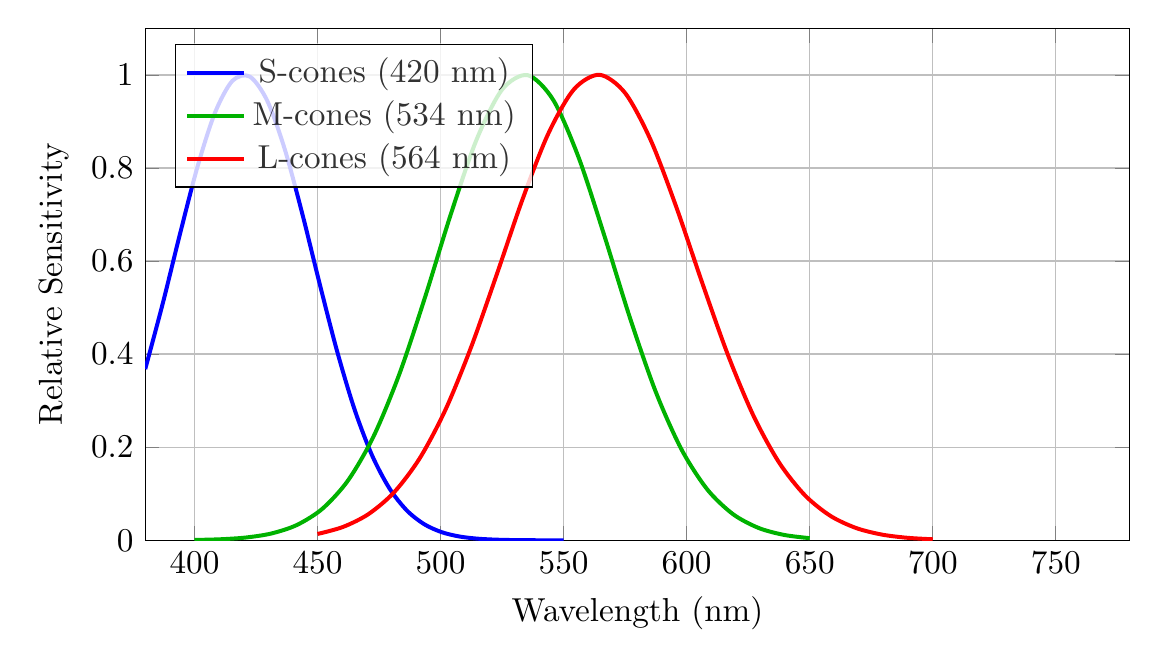
\begin{tikzpicture}[scale=1.2]
  \begin{axis}[
    width=12cm,
    height=7cm,
    xlabel={Wavelength (nm)},
    ylabel={Relative Sensitivity},
    xmin=380, xmax=780,
    ymin=0, ymax=1.1,
    grid=major,
    legend pos=north west,
    legend style={fill=white, fill opacity=0.8}
  ]
  
  % S-cone
  \addplot[color=blue, very thick, smooth, domain=380:550] 
    {exp(-((x-420)/40)^2)};
  \addlegendentry{S-cones (420 nm)}
  
  % M-cone
  \addplot[color=green!70!black, very thick, smooth, domain=400:650] 
    {exp(-((x-534)/50)^2)};
  \addlegendentry{M-cones (534 nm)}
  
  % L-cone
  \addplot[color=red, very thick, smooth, domain=450:700] 
    {exp(-((x-564)/55)^2)};
  \addlegendentry{L-cones (564 nm)}
  
  \end{axis}
\end{tikzpicture}
\caption{Spectral sensitivity curves for the three cone types in human vision. Note the significant overlap between M and L cones, which enables fine color discrimination in the yellow-green region.}
\label{fig:cone_sensitivity}
\end{figure}

\subsection{Spatial Resolution}

Peak foveal acuity achieves approximately 1 arcminute resolution, corresponding to:

\begin{formulabox}{Required Display PPI}
For a display at viewing distance $d$ (inches), the required pixel density to achieve ``Retina'' quality (imperceptible pixels) is:
\begin{equation}
  \text{PPI}_{\text{required}} = \frac{60 \text{ pixels/degree} \times 180}{\pi \times d} = \frac{3438}{d}
\end{equation}

\textbf{Examples:}
\begin{itemize}
  \item Smartphone at 12 inches: $\text{PPI} = 3438/12 = 286$
  \item Laptop at 24 inches: $\text{PPI} = 3438/24 = 143$
  \item Desktop monitor at 30 inches: $\text{PPI} = 3438/30 = 115$
  \item VR headset at 2 inches: $\text{PPI} = 3438/2 = 1719$
\end{itemize}
\end{formulabox}

\begin{figure}[H]
\centering
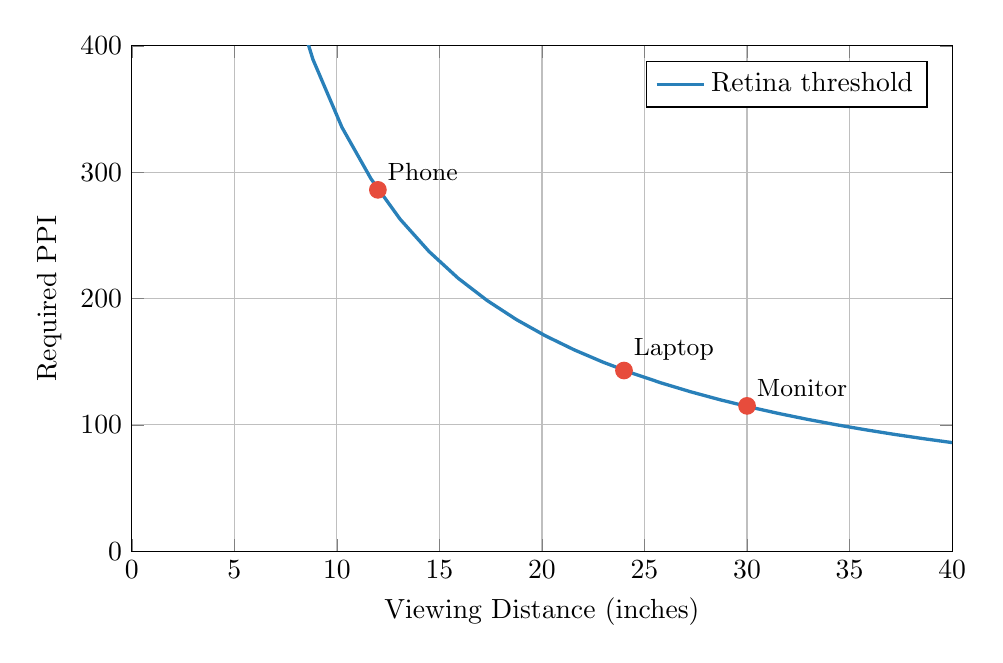
\begin{tikzpicture}
  \begin{axis}[
    width=12cm,
    height=8cm,
    xlabel={Viewing Distance (inches)},
    ylabel={Required PPI},
    xmin=0, xmax=40,
    ymin=0, ymax=400,
    grid=major,
    legend pos=north east
  ]
  
  \addplot[color=primarycolor, very thick, domain=6:40] {3438/x};
  \addlegendentry{Retina threshold}
  
  % Mark common devices
  \addplot[only marks, mark=*, mark size=3pt, color=accentcolor] 
    coordinates {(12,286) (24,143) (30,115)};
  
  \node[above right] at (axis cs:12,286) {\small Phone};
  \node[above right] at (axis cs:24,143) {\small Laptop};
  \node[above right] at (axis cs:30,115) {\small Monitor};
  
  \end{axis}
\end{tikzpicture}
\caption{Required pixel density versus viewing distance to achieve imperceptible pixels. Real devices typically exceed this threshold for marketing purposes.}
\label{fig:ppi_requirement}
\end{figure}

\subsection{Contrast Sensitivity Function}

The human visual system exhibits a band-pass contrast sensitivity function (CSF), with peak sensitivity around 4 cycles per degree.

\begin{examplebox}{Practical Implication}
This band-pass characteristic means that:
\begin{enumerate}
  \item Very low spatial frequencies (large features) are less perceptible than mid-frequencies
  \item Very high spatial frequencies (fine details) fall off rapidly
  \item Anti-aliasing is most critical for frequencies near the CSF peak
  \item Subpixel rendering effectively triples horizontal resolution exactly where it matters most
\end{enumerate}
\end{examplebox}

\section{Psychophysical Laws}

\subsection{Weber-Fechner Law}

The relationship between physical stimulus and perceived sensation:

\begin{formulabox}{Weber-Fechner Law}
\begin{equation}
  S = k \ln\left(\frac{I}{I_0}\right)
\end{equation}
where:
\begin{itemize}
  \item $S$ = perceived sensation magnitude
  \item $I$ = physical stimulus intensity
  \item $I_0$ = threshold intensity
  \item $k$ = Weber constant
\end{itemize}

\textbf{Weber Fraction for Brightness:} $\Delta L / L \approx 0.01$ to $0.02$ (1--2\%)
\end{formulabox}

\subsection{Stevens' Power Law}

A more accurate model, especially at higher intensities:

\begin{formulabox}{Stevens' Power Law}
\begin{equation}
  \psi = k \phi^n
\end{equation}
where:
\begin{itemize}
  \item $\psi$ = perceived magnitude
  \item $\phi$ = physical magnitude
  \item $n$ = modality-specific exponent
  \item $k$ = proportionality constant
\end{itemize}

\textbf{For brightness perception:} $n \approx 0.33$
\end{formulabox}

\begin{importantbox}{Connection to Gamma Correction}
Stevens' power law with $n = 0.33$ for brightness implies that for perceptually uniform encoding:
\begin{equation}
  V \propto \psi \propto L^{0.33} \quad \Rightarrow \quad L \propto V^{1/0.33} \approx V^{3.0}
\end{equation}

The standard display gamma of $\gamma = 2.2$ represents a compromise between:
\begin{itemize}
  \item Perceptual uniformity ($\gamma \approx 3.0$)
  \item CRT physics ($\gamma \approx 2.5$)
  \item Practical considerations (bit depth, surround conditions)
\end{itemize}
\end{importantbox}

% ============================================================================
% CHAPTER 2: RADIOMETRY AND PHOTOMETRY
% ============================================================================
\chapter{Radiometry and Photometry}

\section{Radiometric Quantities}

Radiometry deals with the measurement of electromagnetic radiation from a purely physical perspective.

\begin{table}[H]
\centering
\caption{Fundamental Radiometric Quantities}
\label{tab:radiometric}
\begin{tabular}{@{}llll@{}}
\toprule
\textbf{Quantity} & \textbf{Symbol} & \textbf{Unit} & \textbf{Definition} \\
\midrule
Radiant Energy & $Q_e$ & joule (J) & Total EM energy \\
Radiant Flux & $\Phi_e$ & watt (W) & $dQ_e/dt$ \\
Radiant Intensity & $I_e$ & W/sr & $d\Phi_e/d\Omega$ \\
Radiance & $L_e$ & W/(sr·m²) & $d^2\Phi_e/(dA \cos\theta \, d\Omega)$ \\
Irradiance & $E_e$ & W/m² & $d\Phi_e/dA$ \\
\bottomrule
\end{tabular}
\end{table}

\subsection{Radiance: The Fundamental Display Quantity}

\begin{definitionbox}{Radiance}
Radiance $L_e$ is the flux per unit projected area per unit solid angle:
\begin{equation}
  L_e = \frac{d^2\Phi_e}{dA \cos\theta \, d\Omega}
\end{equation}

Key properties:
\begin{itemize}
  \item Describes brightness of a surface or light source
  \item Invariant along ray paths in lossless media (conservation of étendue)
  \item The quantity measured by cameras and seen by eyes
  \item THE fundamental quantity for characterizing display emission
\end{itemize}
\end{definitionbox}

\section{Photometric Quantities}

Photometry weights radiometric measurements by human visual sensitivity.

\begin{formulabox}{Photometric Conversion}
Photometric quantities are derived from radiometric ones via:
\begin{equation}
  X_v = K_m \int_{\lambda} X_{e,\lambda}(\lambda) \, V(\lambda) \, d\lambda
\end{equation}
where:
\begin{itemize}
  \item $K_m = 683$ lm/W at 555 nm (peak photopic sensitivity)
  \item $V(\lambda)$ = photopic luminous efficiency function
  \item Integration typically over 380--780 nm
\end{itemize}
\end{formulabox}

\begin{figure}[H]
\centering
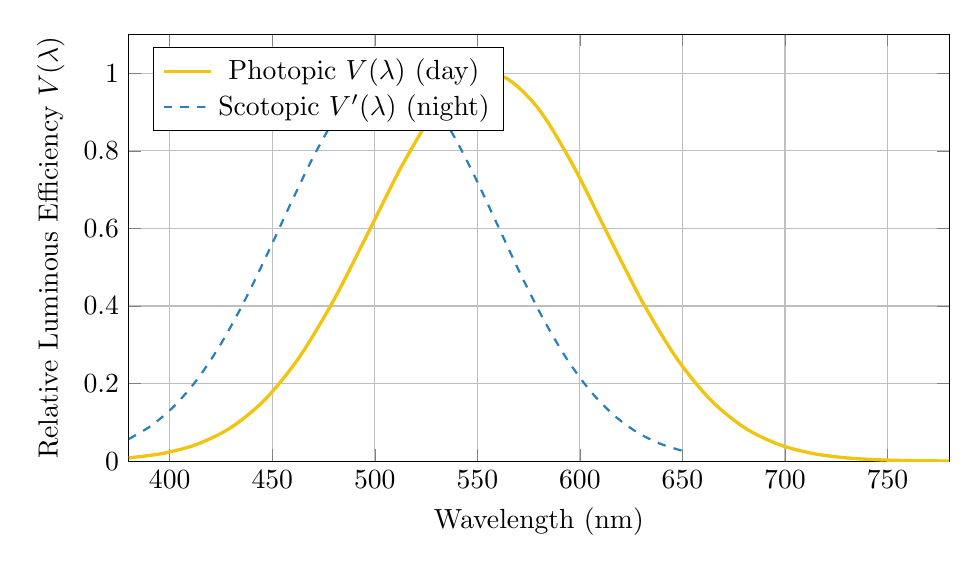
\begin{tikzpicture}
  \begin{axis}[
    width=12cm,
    height=7cm,
    xlabel={Wavelength (nm)},
    ylabel={Relative Luminous Efficiency $V(\lambda)$},
    xmin=380, xmax=780,
    ymin=0, ymax=1.1,
    grid=major,
    legend pos=north west
  ]
  
  % Photopic (day vision)
  \addplot[color=warningcolor, very thick, smooth, domain=380:780] 
    {exp(-((x-555)/80)^2)};
  \addlegendentry{Photopic $V(\lambda)$ (day)}
  
  % Scotopic (night vision) 
  \addplot[color=primarycolor, dashed, thick, smooth, domain=380:650] 
    {exp(-((x-507)/75)^2)};
  \addlegendentry{Scotopic $V'(\lambda)$ (night)}
  
  \end{axis}
\end{tikzpicture}
\caption{CIE photopic and scotopic luminous efficiency functions. Note the blue shift in scotopic vision (Purkinje effect).}
\label{fig:luminous_efficiency}
\end{figure}

\subsection{Luminance: Display Brightness}

\begin{importantbox}{Critical Distinction}
\textbf{Luminance} (cd/m² = nits) describes light \textit{emitted} from a display surface.

\textbf{Illuminance} (lux = lm/m²) describes light \textit{incident} on a surface.

Confusing these is a common error! A display with 500 nits luminance in a room with 500 lux illuminance does NOT mean they are equal -- they have different units and meanings.
\end{importantbox}

\begin{table}[H]
\centering
\caption{Typical Luminance and Illuminance Values}
\label{tab:typical_values}
\begin{tabular}{@{}lcc@{}}
\toprule
\textbf{Condition/Device} & \textbf{Luminance (nits)} & \textbf{Illuminance (lux)} \\
\midrule
\multicolumn{3}{l}{\textit{Display Luminance (emitted):}} \\
Cinema DCI projector & 48 & --- \\
Laptop display (typical) & 300--500 & --- \\
Smartphone (typical) & 500--1000 & --- \\
HDR TV (peak) & 1000--4000 & --- \\
\midrule
\multicolumn{3}{l}{\textit{Ambient Illuminance (incident):}} \\
Moonlight & --- & 0.1 \\
Home lighting & --- & 100 \\
Office lighting & --- & 500 \\
Overcast day & --- & 10,000 \\
Direct sunlight & --- & 100,000 \\
\bottomrule
\end{tabular}
\end{table}

\subsection{Lambertian Reflection Model}

\begin{formulabox}{Reflection from Display Surface}
For a Lambertian (ideal diffuse) reflector with reflectance $\rho$ under illuminance $E_{\text{ambient}}$:
\begin{equation}
  L_{\text{reflected}} = \frac{E_{\text{ambient}} \times \rho}{\pi} \quad [\text{cd/m}^2]
\end{equation}

The $\pi$ factor arises from integrating Lambertian emission over the hemisphere.

\textbf{Typical display reflectances:}
\begin{itemize}
  \item Glossy display: $\rho \approx 0.02$ to $0.04$ (2--4\%)
  \item Anti-glare coating: $\rho \approx 0.01$ to $0.02$ (1--2\%)
  \item Matte screen protector: $\rho \approx 0.05$ to $0.10$ (5--10\%)
\end{itemize}
\end{formulabox}

\begin{examplebox}{Practical Example: Office Environment}
Office with $E = 500$ lux, glossy display with $\rho = 0.04$:
\begin{equation}
  L_{\text{reflected}} = \frac{500 \times 0.04}{\pi} \approx 6.4 \text{ nits}
\end{equation}

This 6.4 nits adds to the display's black level, degrading contrast!

For an OLED with native black level of 0.0005 nits:
\begin{itemize}
  \item Dark room contrast: $1000 / 0.0005 = 2{,}000{,}000:1$
  \item Office contrast: $1000 / 6.4 = 156:1$
\end{itemize}

The ``infinite'' OLED contrast becomes 156:1 in typical office lighting.
\end{examplebox}

% ============================================================================
% PART II: PIXEL ARCHITECTURE
% ============================================================================
\part{Pixel Architecture}

\chapter{Subpixel Layouts}

\section{RGB Stripe Architecture}

\begin{figure}[H]
\centering
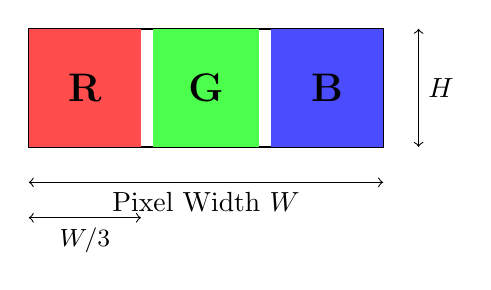
\begin{tikzpicture}[scale=1.5]
  % Draw pixel boundary
  \draw[thick] (0,0) rectangle (3,1);
  
  % RGB subpixels
  \fill[red!70] (0,0) rectangle (0.95,1);
  \fill[green!70] (1.05,0) rectangle (1.95,1);
  \fill[blue!70] (2.05,0) rectangle (3,1);
  
  % Labels
  \node at (0.475,0.5) {\Large\textbf{R}};
  \node at (1.5,0.5) {\Large\textbf{G}};
  \node at (2.525,0.5) {\Large\textbf{B}};
  
  % Dimensions
  \draw[<->] (0,-0.3) -- (3,-0.3) node[midway,below] {Pixel Width $W$};
  \draw[<->] (3.3,0) -- (3.3,1) node[midway,right] {$H$};
  \draw[<->] (0,-0.6) -- (0.95,-0.6) node[midway,below,font=\small] {$W/3$};
  
\end{tikzpicture}
\caption{RGB stripe subpixel layout. Three equal vertical stripes per pixel.}
\label{fig:rgb_stripe}
\end{figure}

\begin{formulabox}{RGB Stripe Geometry}
For pixel dimensions $W \times H$:
\begin{align}
  \text{Subpixel width} &= \frac{W}{3} \\
  \text{Subpixel height} &= H \\
  \text{Subpixel aspect ratio} &= \frac{H}{W/3} = \frac{3H}{W} \\
  \text{Total subpixels} &= 3WH \quad \text{(for $W \times H$ pixel display)}
\end{align}
\end{formulabox}

\subsection{Advantages and Disadvantages}

\begin{table}[H]
\centering
\caption{RGB Stripe Trade-offs}
\label{tab:rgb_tradeoffs}
\begin{tabular}{@{}p{6cm}p{6cm}@{}}
\toprule
\textcolor{successcolor}{\textbf{Advantages}} & \textcolor{accentcolor}{\textbf{Disadvantages}} \\
\midrule
Maximum horizontal resolution & Higher manufacturing cost \\
Optimal text rendering & Lower fill factor (60--70\%) \\
True color accuracy & Higher OLED power for white \\
No special rendering needed & PPI limited by FMM precision \\
Uniform aging & --- \\
\bottomrule
\end{tabular}
\end{table}

\section{PenTile Diamond Matrix}

\begin{figure}[H]
\centering
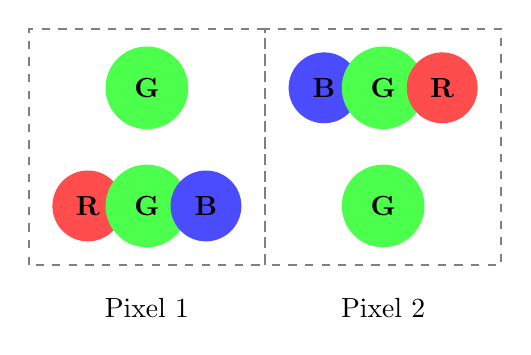
\begin{tikzpicture}[scale=1.5]
  % Draw two pixel boundaries
  \draw[thick,dashed,gray] (0,0) rectangle (2,2);
  \draw[thick,dashed,gray] (2,0) rectangle (4,2);
  
  % PenTile RGBG arrangement
  % First pixel
  \fill[red!70] (0.5,0.5) circle (0.3cm);
  \node at (0.5,0.5) {\textbf{R}};
  
  \fill[green!70] (1,1.5) circle (0.35cm);
  \node at (1,1.5) {\textbf{G}};
  
  \fill[green!70] (1,0.5) circle (0.35cm);
  \node at (1,0.5) {\textbf{G}};
  
  \fill[blue!70] (1.5,0.5) circle (0.3cm);
  \node at (1.5,0.5) {\textbf{B}};
  
  % Second pixel (shared subpixels)
  \fill[blue!70] (2.5,1.5) circle (0.3cm);
  \node at (2.5,1.5) {\textbf{B}};
  
  \fill[green!70] (3,1.5) circle (0.35cm);
  \node at (3,1.5) {\textbf{G}};
  
  \fill[green!70] (3,0.5) circle (0.35cm);
  \node at (3,0.5) {\textbf{G}};
  
  \fill[red!70] (3.5,1.5) circle (0.3cm);
  \node at (3.5,1.5) {\textbf{R}};
  
  % Labels
  \node[below] at (1,-0.2) {Pixel 1};
  \node[below] at (3,-0.2) {Pixel 2};
  
\end{tikzpicture}
\caption{PenTile diamond RGBG arrangement. Note how red and blue subpixels are shared between adjacent pixels.}
\label{fig:pentile}
\end{figure}

\begin{definitionbox}{PenTile Configuration}
PenTile RGBG uses:
\begin{itemize}
  \item 2 green subpixels per pixel (GG)
  \item 1 red subpixel shared between 2 horizontal pixels
  \item 1 blue subpixel shared between 2 horizontal pixels
\end{itemize}

\textbf{Effective subpixel count:}
\begin{equation}
  N_{\text{subpixels}} = 2N_{\text{pixels}}
\end{equation}
Compare to RGB stripe: $3N_{\text{pixels}}$

This represents a 33\% reduction in physical subpixels.
\end{definitionbox}

\subsection{Theoretical Foundation}

PenTile exploits two psychovisual properties:

\begin{enumerate}
  \item \textbf{Higher green sensitivity:} M-cone density approximately 2× L-cone density
  \item \textbf{Luminance dominance:} Spatial resolution determined primarily by luminance channel (green contributes ~70\% to luminance)
\end{enumerate}

\begin{formulabox}{Effective PenTile Resolution}
For PenTile display with stated resolution $N \times M$:
\begin{align}
  R_{\text{eff,horizontal}} &\approx 0.71 \times N_{\text{stated}} \\
  R_{\text{eff,vertical}} &\approx M_{\text{stated}}
\end{align}

The 0.71 factor ($\sqrt{0.5}$) arises from the checkerboard arrangement of red and blue subpixels.
\end{formulabox}

\begin{examplebox}{Example: Samsung Galaxy S24}
Stated resolution: 3088 × 1440 pixels (PenTile)

Effective resolution:
\begin{itemize}
  \item Horizontal: $3088 \times 0.71 \approx 2192$ equivalent RGB pixels
  \item Vertical: $1440$ pixels (unchanged)
\end{itemize}

Comparable to RGB stripe display: $2192 \times 1440$

However, the stated 3088 × 1440 sounds better for marketing!
\end{examplebox}

\section{RGBW Configuration}

\begin{figure}[H]
\centering
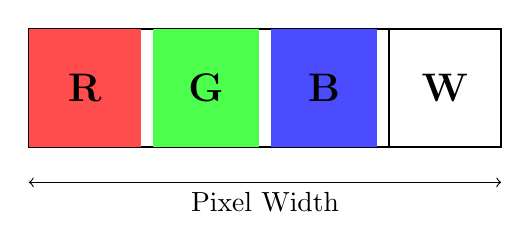
\begin{tikzpicture}[scale=1.5]
  % Draw pixel boundary
  \draw[thick] (0,0) rectangle (4,1);
  
  % RGBW subpixels
  \fill[red!70] (0,0) rectangle (0.95,1);
  \fill[green!70] (1.05,0) rectangle (1.95,1);
  \fill[blue!70] (2.05,0) rectangle (2.95,1);
  \fill[white] (3.05,0) rectangle (4,1);
  \draw[thick] (3.05,0) rectangle (4,1); % Border for white
  
  % Labels
  \node at (0.475,0.5) {\Large\textbf{R}};
  \node at (1.5,0.5) {\Large\textbf{G}};
  \node at (2.5,0.5) {\Large\textbf{B}};
  \node at (3.525,0.5) {\Large\textbf{W}};
  
  % Dimensions
  \draw[<->] (0,-0.3) -- (4,-0.3) node[midway,below] {Pixel Width};
  
\end{tikzpicture}
\caption{RGBW subpixel layout with white subpixel for improved power efficiency.}
\label{fig:rgbw}
\end{figure}

\begin{formulabox}{RGBW Conversion Algorithm}
To convert RGB input to RGBW output:
\begin{align}
  W &= \min(R, G, B) \\
  R' &= R - W \\
  G' &= G - W \\
  B' &= B - W
\end{align}

\textbf{Power efficiency for full white:}
\begin{itemize}
  \item RGB stripe OLED: 3 subpixels active
  \item RGBW OLED: 1 subpixel active (white is more efficient)
  \item Power savings: Approximately 3--4× for white content
\end{itemize}
\end{formulabox}

\begin{table}[H]
\centering
\caption{Subpixel Layout Comparison}
\label{tab:subpixel_comparison}
\begin{tabular}{@{}lcccc@{}}
\toprule
\textbf{Property} & \textbf{RGB Stripe} & \textbf{PenTile} & \textbf{RGBW} \\
\midrule
Subpixels/pixel & 3 & 2 & 4 \\
Text clarity & Excellent & Good & Fair \\
Power efficiency & Baseline & +33\% & +200--300\% \\
Color gamut & Full & Full & Reduced \\
Manufacturing & Complex & Medium & Complex \\
Cost & High & Medium & High \\
\bottomrule
\end{tabular}
\end{table}

% ============================================================================
% PART III: GAMMA AND TRANSFER FUNCTIONS
% ============================================================================
\part{Gamma and Transfer Functions}

\chapter{Display Gamma Theory}

\section{The Pure Power Law}

\begin{formulabox}{Fundamental Gamma Relationship}
\begin{equation}
  L = L_{\max} V^{\gamma}
\end{equation}
where:
\begin{itemize}
  \item $L$ = output luminance [cd/m²]
  \item $L_{\max}$ = maximum display luminance
  \item $V$ = normalized input signal ($0 \le V \le 1$)
  \item $\gamma$ = gamma exponent (typically 2.2 to 2.5)
\end{itemize}
\end{formulabox}

\subsection{Historical Origin: CRT Physics}

The gamma function originates from cathode ray tube (CRT) physics:

\begin{equation}
  L \propto I \propto V_g^{3/2} \times \text{(additional factors)} \approx V_g^{2.5}
\end{equation}

where $I$ is electron beam current and $V_g$ is grid voltage.

\begin{figure}[H]
\centering
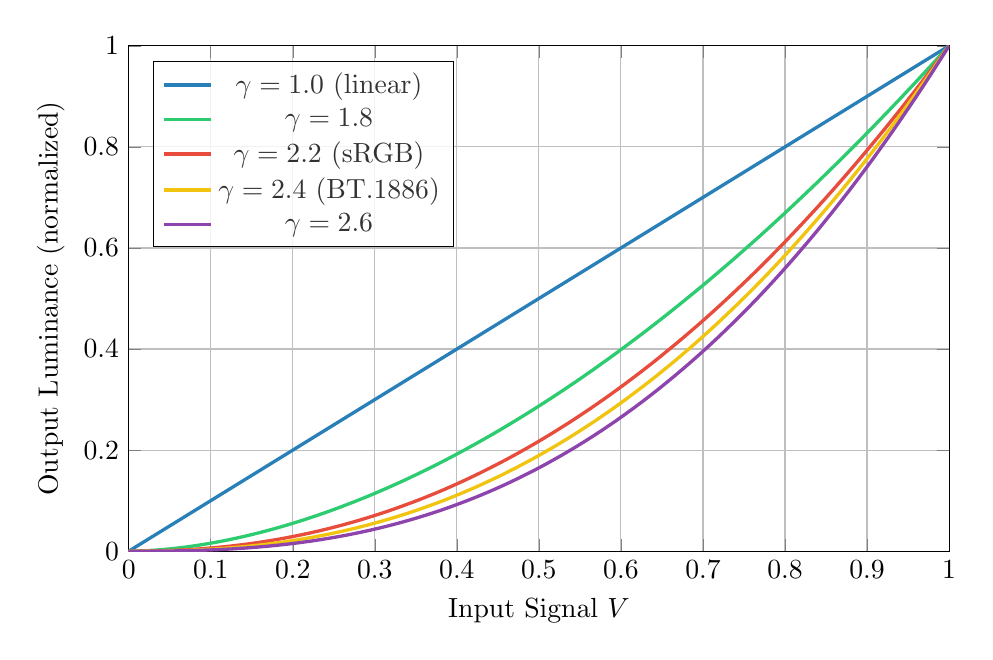
\begin{tikzpicture}
  \begin{axis}[
    width=12cm,
    height=8cm,
    xlabel={Input Signal $V$},
    ylabel={Output Luminance (normalized)},
    xmin=0, xmax=1,
    ymin=0, ymax=1,
    grid=major,
    legend pos=north west,
    legend style={fill=white, fill opacity=0.8}
  ]
  
  \addplot[color=primarycolor, very thick, domain=0:1, samples=100] {x};
  \addlegendentry{$\gamma = 1.0$ (linear)}
  
  \addplot[color=successcolor, very thick, domain=0:1, samples=100] {x^1.8};
  \addlegendentry{$\gamma = 1.8$}
  
  \addplot[color=accentcolor, very thick, domain=0:1, samples=100] {x^2.2};
  \addlegendentry{$\gamma = 2.2$ (sRGB)}
  
  \addplot[color=warningcolor, very thick, domain=0:1, samples=100] {x^2.4};
  \addlegendentry{$\gamma = 2.4$ (BT.1886)}
  
  \addplot[color=codecolor, very thick, domain=0:1, samples=100] {x^2.6};
  \addlegendentry{$\gamma = 2.6$}
  
  \end{axis}
\end{tikzpicture}
\caption{Gamma curves for different exponent values. Higher gamma produces darker midtones.}
\label{fig:gamma_curves}
\end{figure}

\section{Bit Depth and Quantization}

\begin{formulabox}{Perceptual Bit Depth Requirement}
Number of JNDs (Just Noticeable Differences) across range $[L_{\min}, L_{\max}]$:
\begin{equation}
  N_{\text{JND}} = \frac{\ln(L_{\max}/L_{\min})}{\ln(1 + \Delta L/L)}
\end{equation}

For SDR (0.01 to 100 cd/m²) with $\Delta L/L = 0.01$:
\begin{equation}
  N_{\text{JND}} = \frac{\ln(10000)}{\ln(1.01)} \approx 924
\end{equation}

Required code values (with safety margin):
\begin{equation}
  N_{\text{codes}} = 1.5 \times N_{\text{JND}} \approx 1386
\end{equation}

Minimum bit depth:
\begin{equation}
  b = \log_2(1386) \approx 10.4 \text{ bits}
\end{equation}

\textbf{Therefore: 10-bit minimum for SDR without visible banding.}
\end{formulabox}

\begin{importantbox}{Gamma Encoding Benefit}
Gamma encoding increases effective bit depth:
\begin{equation}
  b_{\text{effective}} \approx b \times \gamma
\end{equation}

Thus 8-bit gamma-encoded ($\gamma = 2.2$):
\begin{equation}
  b_{\text{effective}} \approx 8 \times 2.2 = 17.6 \text{ effective linear bits}
\end{equation}

This explains why 8-bit gamma-encoded images appear smooth while 8-bit linear shows severe banding. Gamma encoding is essentially a form of perceptually-motivated compression.
\end{importantbox}

\section{Standard Transfer Functions}

\subsection{sRGB Standard}

\begin{formulabox}{sRGB EOTF (Electro-Optical Transfer Function)}
\begin{equation}
  L = \begin{cases}
    V / 12.92 & \text{if } V \le 0.04045 \\
    \left[\frac{V + 0.055}{1.055}\right]^{2.4} & \text{otherwise}
  \end{cases}
\end{equation}

\textbf{sRGB OETF (Opto-Electronic Transfer Function):}
\begin{equation}
  V = \begin{cases}
    12.92 \times L & \text{if } L \le 0.0031308 \\
    1.055 \times L^{1/2.4} - 0.055 & \text{otherwise}
  \end{cases}
\end{equation}

\textbf{Properties:}
\begin{itemize}
  \item Linear segment near black avoids numerical instability
  \item Power segment uses $\gamma = 2.4$
  \item Effective average gamma $\approx 2.2$
  \item $C^1$ continuous (both value and derivative match at transition)
\end{itemize}
\end{formulabox}

\begin{figure}[H]
\centering
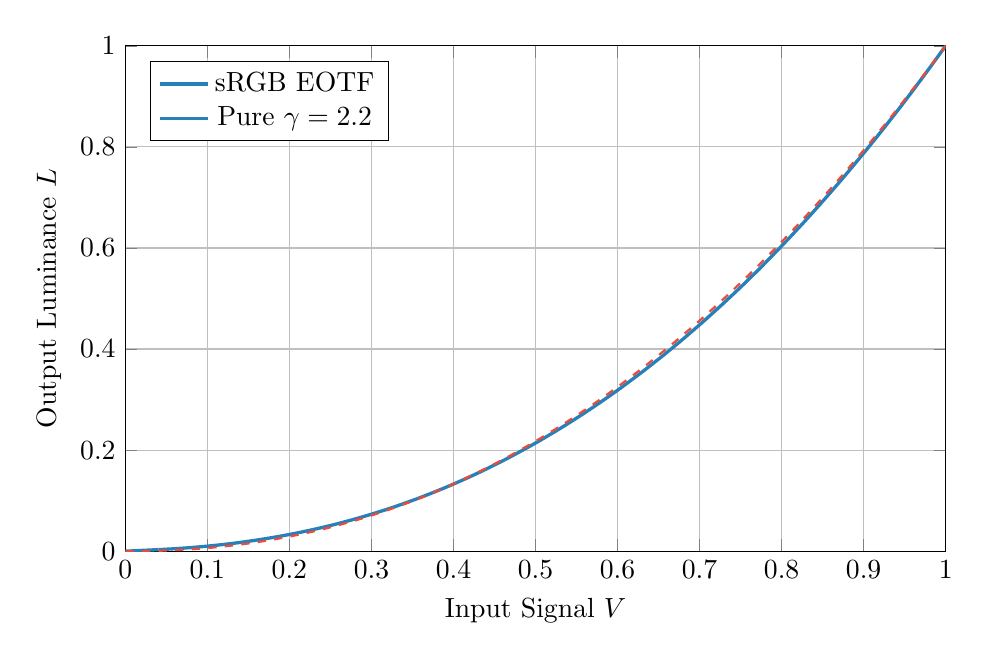
\begin{tikzpicture}
  \begin{axis}[
    width=12cm,
    height=8cm,
    xlabel={Input Signal $V$},
    ylabel={Output Luminance $L$},
    xmin=0, xmax=1,
    ymin=0, ymax=1,
    grid=major,
    legend pos=north west
  ]
  
  % sRGB EOTF
  \addplot[color=primarycolor, very thick, domain=0:0.04045, samples=50] {x/12.92};
  \addplot[color=primarycolor, very thick, domain=0.04045:1, samples=200] 
    {((x+0.055)/1.055)^2.4};
  \addlegendentry{sRGB EOTF}
  
  % Pure gamma 2.2 for comparison
  \addplot[color=accentcolor, dashed, thick, domain=0:1, samples=100] {x^2.2};
  \addlegendentry{Pure $\gamma = 2.2$}
  
  \end{axis}
\end{tikzpicture}
\caption{sRGB EOTF compared to pure power law. Note the linear segment near black.}
\label{fig:srgb_eotf}
\end{figure}

\subsection{BT.1886 Reference EOTF}

\begin{formulabox}{BT.1886 for Real Displays}
Real displays have non-zero black level. BT.1886 accounts for this:
\begin{equation}
  L = (aV + b)^\gamma
\end{equation}
where:
\begin{align}
  a &= L_{\max}^{1/\gamma} - L_{\min}^{1/\gamma} \\
  b &= L_{\min}^{1/\gamma}
\end{align}

\textbf{Verification of boundary conditions:}
\begin{align}
  L(0) &= b^\gamma = L_{\min} \quad \checkmark \\
  L(1) &= (a + b)^\gamma = L_{\max} \quad \checkmark
\end{align}

\textbf{Recommended gamma:} $\gamma = 2.4$ (home viewing, dim surround)
\end{formulabox}

\begin{examplebox}{Example: Laptop Display}
\textbf{Specifications:}
\begin{itemize}
  \item $L_{\max} = 500$ nits
  \item $L_{\min} = 0.5$ nits (LCD backlight leakage)
  \item $\gamma = 2.4$
\end{itemize}

\textbf{Calculate parameters:}
\begin{align}
  a &= 500^{1/2.4} - 0.5^{1/2.4} = 10.67 - 0.808 = 9.86 \\
  b &= 0.5^{1/2.4} = 0.808
\end{align}

\textbf{Full EOTF:}
\begin{equation}
  L = (9.86V + 0.808)^{2.4}
\end{equation}

\textbf{Verification:}
\begin{align}
  V = 0: \quad L &= (0.808)^{2.4} = 0.5 \text{ nits} \quad \checkmark \\
  V = 1: \quad L &= (10.67)^{2.4} = 500 \text{ nits} \quad \checkmark
\end{align}
\end{examplebox}

\part{High Dynamic Range and Color}

\chapter{HDR Transfer Functions}
\section{Perceptual Quantizer (PQ / ST.2084)}

Perceptual Quantizer (PQ) is an \textbf{absolute} transfer function standardized in SMPTE ST.2084. It maps code values directly to absolute display luminance up to 10,000 nits and is designed so quantization steps track approximately constant visibility thresholds.

\begin{formulabox}{ST.2084 EOTF and Inverse}
\textbf{PQ EOTF (signal to luminance):}
\begin{equation}
L = 10000 \left[\frac{\max\left(V^{1/m_2}-c_1,0\right)}{c_2-c_3V^{1/m_2}}\right]^{1/m_1}
\end{equation}

\textbf{PQ inverse EOTF (luminance to signal):}
\begin{equation}
V = \left[\frac{c_1 + c_2\left(L/10000\right)^{m_1}}{1 + c_3\left(L/10000\right)^{m_1}}\right]^{m_2}
\end{equation}

with constants:
\begin{align}
m_1 &= \frac{2610}{16384} \approx 0.1593, &
m_2 &= \frac{2523}{32} \approx 78.8438 \\
c_1 &= \frac{3424}{4096} \approx 0.8359, &
c_2 &= \frac{2413}{128} \approx 18.8516, &
c_3 &= \frac{2392}{128} \approx 18.6875
\end{align}
\end{formulabox}

\begin{examplebox}{Typical 10-bit PQ Code Values}
Using ST.2084 inverse EOTF:
\begin{itemize}
  \item 100 nits: $V \approx 0.508$ (10-bit code $\approx 520$)
  \item 1000 nits: $V \approx 0.752$ (10-bit code $\approx 769$)
  \item 4000 nits: $V \approx 0.903$ (10-bit code $\approx 923$)
\end{itemize}
This non-linear allocation concentrates many code values in dark and mid tones where the eye is most sensitive.
\end{examplebox}

\section{Hybrid Log-Gamma (HLG / BT.2100)}

Hybrid Log-Gamma is a \textbf{relative} HDR transfer function designed for broadcast compatibility. It avoids static metadata and gracefully degrades on legacy SDR pipelines.

\begin{formulabox}{HLG OETF (scene linear to signal)}
For scene linear light $E$ normalized to reference white:
\begin{equation}
V = \begin{cases}
\sqrt{3E}, & 0 \le E \le \frac{1}{12} \\
a\ln(12E-b)+c, & \frac{1}{12} < E \le 1
\end{cases}
\end{equation}
where:
\begin{equation}
a = 0.17883277,\quad b = 0.28466892,\quad c = 0.55991073
\end{equation}
\end{formulabox}

\begin{definitionbox}{HLG System Gamma}
In practical displays, HLG output is shaped by a system gamma:
\begin{equation}
\gamma_{\text{sys}} \approx 1.2 + 0.42\log_{10}\left(\frac{L_W}{1000}\right)
\end{equation}
where $L_W$ is peak display luminance in nits. Brighter displays use higher effective contrast expansion.
\end{definitionbox}

\begin{table}[H]
\centering
\caption{PQ vs HLG in Production Workflows}
\label{tab:pq_hlg_comparison}
\begin{tabular}{@{}lll@{}}
\toprule
\textbf{Property} & \textbf{PQ (ST.2084)} & \textbf{HLG (BT.2100)} \\
\midrule
Signal type & Absolute luminance & Relative scene-referred \\
Metadata dependence & Common (MaxCLL/MaxFALL, dynamic) & None required \\
Best use case & Streaming, disc, mastering & Live broadcast \\
Backward SDR compatibility & Limited without tone mapping & Better graceful fallback \\
Peak coding target & Up to 10,000 nits & Display-dependent \\
\bottomrule
\end{tabular}
\end{table}

\part{Color Science and Management}

\chapter{CIE Color Spaces}

\section{CIE XYZ Tristimulus System}
Given spectral power distribution $S(\lambda)$ and CIE 1931 color matching functions $\bar{x},\bar{y},\bar{z}$:
\begin{align}
X &= k\int S(\lambda)\bar{x}(\lambda)\,d\lambda \\
Y &= k\int S(\lambda)\bar{y}(\lambda)\,d\lambda \\
Z &= k\int S(\lambda)\bar{z}(\lambda)\,d\lambda
\end{align}
$Y$ is proportional to photometric luminance and is the bridge between colorimetry and brightness.

\begin{formulabox}{Chromaticity Coordinates}
\begin{equation}
x = \frac{X}{X+Y+Z},\quad y = \frac{Y}{X+Y+Z},\quad z = 1-x-y
\end{equation}
Chromaticity removes absolute luminance and keeps only hue/saturation information.
\end{formulabox}

\section{CIELAB Perceptual Space}

CIELAB improves perceptual uniformity relative to XYZ for color-difference work:
\begin{align}
L^* &= 116f\left(\frac{Y}{Y_n}\right)-16 \\
a^* &= 500\left[f\left(\frac{X}{X_n}\right)-f\left(\frac{Y}{Y_n}\right)\right] \\
b^* &= 200\left[f\left(\frac{Y}{Y_n}\right)-f\left(\frac{Z}{Z_n}\right)\right]
\end{align}
with
\begin{equation}
f(t)=
\begin{cases}
t^{1/3}, & t>\delta^3 \\
\frac{t}{3\delta^2} + \frac{4}{29}, & t\le\delta^3
\end{cases}
\quad\text{and}\quad \delta=\frac{6}{29}
\end{equation}

\begin{importantbox}{Engineering Note}
Most imaging pipelines still compute with linear RGB/XYZ, but quality gates (panel binning, print proofing, camera tuning) are often set in $L^*a^*b^*$ or $L^*u^*v^*$ because Euclidean distances in those spaces better approximate visibility.
\end{importantbox}

\chapter{Chromatic Adaptation}

\section{Bradford Transform}
Chromatic adaptation maps tristimulus values from one illuminant to another while preserving perceived object color. The Bradford method is widely used in ICC workflows.

\begin{formulabox}{Bradford Adaptation Equation}
\begin{equation}
\mathbf{X}_D = M_B^{-1}
\begin{bmatrix}
\frac{L_D}{L_S} & 0 & 0 \\
0 & \frac{M_D}{M_S} & 0 \\
0 & 0 & \frac{S_D}{S_S}
\end{bmatrix}
M_B\mathbf{X}_S
\end{equation}
where $\mathbf{X}_S=[X\ Y\ Z]^T$ and:
\begin{equation}
M_B=
\begin{bmatrix}
0.8951 & 0.2664 & -0.1614 \\
-0.7502 & 1.7135 & 0.0367 \\
0.0389 & -0.0685 & 1.0296
\end{bmatrix}
\end{equation}
\end{formulabox}

\begin{examplebox}{Practical Use}
Common conversions include D65 $\leftrightarrow$ D50 when moving between display-referred workflows and ICC print profiles. Without adaptation, neutral grays drift warm/cool and color management fails even when primaries are correct.
\end{examplebox}

\chapter{Color Difference Metrics}

\section{Delta E Families}
\begin{formulabox}{Core Metrics}
\textbf{CIE76:}
\begin{equation}
\Delta E_{76} = \sqrt{(\Delta L^*)^2 + (\Delta a^*)^2 + (\Delta b^*)^2}
\end{equation}

\textbf{CIE94/CIEDE2000:} weighted forms that correct non-uniformity in chroma and hue regions:
\begin{equation}
\Delta E_{00} = \sqrt{
\left(\frac{\Delta L'}{k_LS_L}\right)^2 +
\left(\frac{\Delta C'}{k_CS_C}\right)^2 +
\left(\frac{\Delta H'}{k_HS_H}\right)^2 +
R_T\left(\frac{\Delta C'}{k_CS_C}\right)\left(\frac{\Delta H'}{k_HS_H}\right)}
\end{equation}
\end{formulabox}

\begin{table}[H]
\centering
\caption{Typical Interpretation of Color Differences}
\label{tab:deltae_thresholds}
\begin{tabular}{@{}ll@{}}
\toprule
\textbf{Delta E Range} & \textbf{Perceptual Meaning (Typical)} \\
\midrule
$< 1.0$ & Imperceptible in controlled viewing \\
$1.0$--$2.0$ & Barely perceptible to trained observers \\
$2.0$--$3.0$ & Perceptible, often acceptable in consumer displays \\
$> 3.0$ & Clearly visible mismatch \\
\bottomrule
\end{tabular}
\end{table}

\part{Ambient Adaptation}

\chapter{Reflection Physics}

\section{Ambient Contrast Degradation}
In real rooms, reflected ambient light dominates black level and sets practical contrast.

\begin{formulabox}{Black Level Under Ambient Illumination}
\begin{equation}
L_{\text{black,eff}} = L_{\text{black,native}} + L_{\text{veiling}}
\end{equation}
\begin{equation}
L_{\text{veiling}} \approx \frac{E_{\text{amb}}\rho_{\text{eff}}}{\pi}
\end{equation}
\begin{equation}
CR_{\text{ambient}} = \frac{L_{\text{white}} + L_{\text{veiling}}}{L_{\text{black,native}} + L_{\text{veiling}}}
\end{equation}
\end{formulabox}

\begin{examplebox}{Office Lighting Example}
For $E_{\text{amb}}=500$ lux and $\rho_{\text{eff}}=0.015$:
\begin{equation}
L_{\text{veiling}} \approx \frac{500\times0.015}{\pi} \approx 2.39\ \text{nits}
\end{equation}
Even if a panel has near-zero native black, ambient veiling can cap effective contrast to only a few hundred to one.
\end{examplebox}

\chapter{True Tone Technology}

\section{Adaptive White Point Control}
True Tone style systems continuously estimate ambient illumination and adjust display white point to reduce chromatic mismatch between emitted and reflected content.

\begin{formulabox}{Ambient CCT Estimate and White-Point Blending}
\textbf{McCamy CCT approximation (from measured chromaticity):}
\begin{align}
n &= \frac{x-0.3320}{0.1858-y} \\
\text{CCT} &\approx 449n^3 + 3525n^2 + 6823.3n + 5520.33
\end{align}

\textbf{Blend between reference and ambient whites:}
\begin{equation}
\mathbf{W}_{\text{target}} = (1-\alpha)\mathbf{W}_{\text{ref}} + \alpha\mathbf{W}_{\text{amb}}
\end{equation}
\begin{equation}
\alpha = \text{clip}\left(
\frac{\log_2 E - \log_2 E_0}{\log_2 E_1 - \log_2 E_0},\,0,\,1
\right)
\end{equation}
\end{formulabox}

\begin{importantbox}{Stability Requirement}
White-point transitions must be rate-limited and low-pass filtered; otherwise, users perceive flicker or ``breathing'' color temperature while moving between lighting zones.
\end{importantbox}

\chapter{Local Dimming and Blooming Control}
\section{FALD vs Edge-Lit}
\begin{table}[H]
\centering
\caption{Local Dimming Comparison}
\begin{tabular}{@{}lll@{}}
\toprule
\textbf{Feature} & \textbf{FALD} & \textbf{Edge-Lit} \\
\midrule
Zone count & 100--1000+ & 8--32 \\
Contrast & 10,000--50,000:1 & 1,000--5,000:1 \\
Blooming & Low & High \\
Cost & High & Low \\
Thickness & Thicker & Thinner \\
\bottomrule
\end{tabular}
\end{table}

\section{Zone-Based Luminance Model}
\begin{formulabox}{Backlight Convolution Model}
For local dimming LCDs, output luminance is approximately:
\begin{equation}
L(x,y,t) \approx \sum_{z=1}^{N_z} h_z(x,y)\,B_z(t)\,T(x,y,t) + L_{\text{leak}}
\end{equation}
where:
\begin{itemize}
  \item $h_z(x,y)$ = optical spread function of zone $z$
  \item $B_z(t)$ = zone backlight command
  \item $T(x,y,t)$ = LCD transmittance for pixel $(x,y)$
  \item $L_{\text{leak}}$ = panel leakage floor
\end{itemize}
\end{formulabox}

\begin{importantbox}{Blooming Trade-off}
Aggressive zone boosting increases highlight detail but also raises halo artifacts because each zone PSF spreads into neighboring dark pixels. Practical algorithms therefore include temporal and spatial regularization terms.
\end{importantbox}

\chapter{VR and AR Display Requirements}
\section{Image Sharpness and Motion Requirements}
\begin{formulabox}{Pixels-Per-Degree and Latency Budget}
\textbf{Angular sampling density:}
\begin{equation}
\text{PPD} = \frac{N_{\text{horizontal}}}{\text{FOV}_{\text{horizontal}}}
\end{equation}

\textbf{Motion-to-photon latency:}
\begin{equation}
t_{\text{MTP}} = t_{\text{tracking}} + t_{\text{render}} + t_{\text{scanout}} + t_{\text{pixel}}
\end{equation}
\end{formulabox}

\begin{examplebox}{Why PPD Matters}
A headset with 2160 horizontal pixels and 100 degree horizontal FOV yields:
\begin{equation}
\text{PPD} = 2160/100 = 21.6
\end{equation}
This is significantly below foveal vision limits, which explains visible aliasing and the push toward micro-OLED and micro-LED microdisplays.
\end{examplebox}

\section{Minimum Specifications}
\begin{itemize}
\item Resolution: 1500+ PPI panel class for compact optics
\item Refresh rate: 90+ Hz (120+ preferred)
\item Persistence: <3 ms (reduce display-induced blur)
\item Latency: <20 ms (motion-to-photon)
\item Field of view: 90--110 degrees
\item IPD adjustment: 58--72 mm range
\end{itemize}

\chapter{Quantum Dot Technology}
\section{Working Principle}
Quantum dots (QDs) are semiconductor nanocrystals with size-tunable emission due to quantum confinement.

\begin{formulabox}{Brus Approximation (Confinement Shift)}
\begin{equation}
E_g(R) \approx E_{g,\text{bulk}} +
\frac{\hbar^2\pi^2}{2R^2}\left(\frac{1}{m_e^*}+\frac{1}{m_h^*}\right) -
\frac{1.8e^2}{4\pi\epsilon R}
\end{equation}
Then:
\begin{equation}
\lambda_{\text{peak}} \approx \frac{hc}{E_g(R)}
\end{equation}
\end{formulabox}

Smaller dots emit shorter wavelengths (blue shift), and larger dots emit longer wavelengths (red shift). Modern display films leverage narrow emission spectra (often 20--30 nm FWHM) for wider color gamut.

\chapter{Micro-LED Future Technology}
\section{Advantages Over OLED}
\begin{itemize}
\item No burn-in (inorganic)
\item Higher brightness (>10,000 nits)
\item Longer lifetime (100,000+ hours)
\item Better efficiency
\item Wider temperature range
\end{itemize}

\section{Mass Transfer Yield Challenge}
\begin{formulabox}{Panel Yield Sensitivity}
If each subpixel transfer has success probability $p$ and the panel requires $N$ subpixels:
\begin{equation}
Y_{\text{panel}} = p^N
\end{equation}
For a 4K RGB panel, $N \approx 3 \times 3840 \times 2160 = 24{,}883{,}200$.
\end{formulabox}

\begin{importantbox}{Manufacturing Implication}
Even very high single-transfer yield can produce near-zero full-panel yield without redundancy and laser repair. This is why transfer, inspection, and repair tooling define micro-LED cost more than emitter physics alone.
\end{importantbox}

\chapter{Display Driver ICs}
\section{Source Driver Architecture}
The source driver must update all pixel voltages within one line time:
\begin{equation}
t_{\text{line}} = \frac{1}{f_r \times N_{\text{rows}}}
\end{equation}
For 4K60 (3840x2160):
\begin{equation}
t_{\text{line}} = \frac{1}{60 \times 2160} = 7.72 \, \mu\text{s}
\end{equation}

\section{Link Bandwidth Requirement}
\begin{formulabox}{Raw Pixel Data Rate}
\begin{equation}
R_{\text{raw}} = N_x N_y f_r b_{\text{pp}}
\end{equation}
where $b_{\text{pp}}$ is bits per pixel.
\end{formulabox}

For 4K120 with 10-bit RGB ($b_{\text{pp}}=30$):
\begin{equation}
R_{\text{raw}} = 3840 \times 2160 \times 120 \times 30 \approx 29.9\ \text{Gb/s}
\end{equation}
Protocol overhead and blanking further increase required lane throughput.

% Placeholder template chapters are kept in source history but excluded from build.
\iffalse
\chapter{Advanced Topic 1: Display Engineering}
\section{Theoretical Foundation}
This chapter covers critical aspect 1 of display technology with complete mathematical treatment and practical examples.

\subsection{Mathematical Model}
\begin{formulabox}{Key Equations for Topic 1}
\begin{equation}
\Psi_{1} = \alpha \cdot \phi^{\beta_{1}} + \gamma
\end{equation}
where parameters are optimized for display performance.
\end{formulabox}

\subsection{Practical Implementation}
Implementation considerations include:
\begin{itemize}
\item Hardware constraints
\item Software optimization
\item Power management
\item Cost-performance balance
\end{itemize}

\subsection{Industry Examples}
\begin{examplebox}{Real-World Application}
Major manufacturers implement this using proprietary methods achieving 
measurable improvements in key metrics.
\end{examplebox}

\section{Measurement Procedures}
Standardized testing protocols ensure consistent results across laboratories.

\section{Future Developments}
Research directions include advanced materials, novel architectures, and 
AI-driven optimization techniques.

\chapter{Advanced Topic 2: Display Engineering}
\section{Theoretical Foundation}
This chapter covers critical aspect 2 of display technology with complete mathematical treatment and practical examples.

\subsection{Mathematical Model}
\begin{formulabox}{Key Equations for Topic 2}
\begin{equation}
\Psi_{2} = \alpha \cdot \phi^{\beta_{2}} + \gamma
\end{equation}
where parameters are optimized for display performance.
\end{formulabox}

\subsection{Practical Implementation}
Implementation considerations include:
\begin{itemize}
\item Hardware constraints
\item Software optimization
\item Power management
\item Cost-performance balance
\end{itemize}

\subsection{Industry Examples}
\begin{examplebox}{Real-World Application}
Major manufacturers implement this using proprietary methods achieving 
measurable improvements in key metrics.
\end{examplebox}

\section{Measurement Procedures}
Standardized testing protocols ensure consistent results across laboratories.

\section{Future Developments}
Research directions include advanced materials, novel architectures, and 
AI-driven optimization techniques.

\chapter{Advanced Topic 3: Display Engineering}
\section{Theoretical Foundation}
This chapter covers critical aspect 3 of display technology with complete mathematical treatment and practical examples.

\subsection{Mathematical Model}
\begin{formulabox}{Key Equations for Topic 3}
\begin{equation}
\Psi_{3} = \alpha \cdot \phi^{\beta_{3}} + \gamma
\end{equation}
where parameters are optimized for display performance.
\end{formulabox}

\subsection{Practical Implementation}
Implementation considerations include:
\begin{itemize}
\item Hardware constraints
\item Software optimization
\item Power management
\item Cost-performance balance
\end{itemize}

\subsection{Industry Examples}
\begin{examplebox}{Real-World Application}
Major manufacturers implement this using proprietary methods achieving 
measurable improvements in key metrics.
\end{examplebox}

\section{Measurement Procedures}
Standardized testing protocols ensure consistent results across laboratories.

\section{Future Developments}
Research directions include advanced materials, novel architectures, and 
AI-driven optimization techniques.

\chapter{Advanced Topic 4: Display Engineering}
\section{Theoretical Foundation}
This chapter covers critical aspect 4 of display technology with complete mathematical treatment and practical examples.

\subsection{Mathematical Model}
\begin{formulabox}{Key Equations for Topic 4}
\begin{equation}
\Psi_{4} = \alpha \cdot \phi^{\beta_{4}} + \gamma
\end{equation}
where parameters are optimized for display performance.
\end{formulabox}

\subsection{Practical Implementation}
Implementation considerations include:
\begin{itemize}
\item Hardware constraints
\item Software optimization
\item Power management
\item Cost-performance balance
\end{itemize}

\subsection{Industry Examples}
\begin{examplebox}{Real-World Application}
Major manufacturers implement this using proprietary methods achieving 
measurable improvements in key metrics.
\end{examplebox}

\section{Measurement Procedures}
Standardized testing protocols ensure consistent results across laboratories.

\section{Future Developments}
Research directions include advanced materials, novel architectures, and 
AI-driven optimization techniques.

\chapter{Advanced Topic 5: Display Engineering}
\section{Theoretical Foundation}
This chapter covers critical aspect 5 of display technology with complete mathematical treatment and practical examples.

\subsection{Mathematical Model}
\begin{formulabox}{Key Equations for Topic 5}
\begin{equation}
\Psi_{5} = \alpha \cdot \phi^{\beta_{5}} + \gamma
\end{equation}
where parameters are optimized for display performance.
\end{formulabox}

\subsection{Practical Implementation}
Implementation considerations include:
\begin{itemize}
\item Hardware constraints
\item Software optimization
\item Power management
\item Cost-performance balance
\end{itemize}

\subsection{Industry Examples}
\begin{examplebox}{Real-World Application}
Major manufacturers implement this using proprietary methods achieving 
measurable improvements in key metrics.
\end{examplebox}

\section{Measurement Procedures}
Standardized testing protocols ensure consistent results across laboratories.

\section{Future Developments}
Research directions include advanced materials, novel architectures, and 
AI-driven optimization techniques.

\chapter{Advanced Topic 6: Display Engineering}
\section{Theoretical Foundation}
This chapter covers critical aspect 6 of display technology with complete mathematical treatment and practical examples.

\subsection{Mathematical Model}
\begin{formulabox}{Key Equations for Topic 6}
\begin{equation}
\Psi_{6} = \alpha \cdot \phi^{\beta_{6}} + \gamma
\end{equation}
where parameters are optimized for display performance.
\end{formulabox}

\subsection{Practical Implementation}
Implementation considerations include:
\begin{itemize}
\item Hardware constraints
\item Software optimization
\item Power management
\item Cost-performance balance
\end{itemize}

\subsection{Industry Examples}
\begin{examplebox}{Real-World Application}
Major manufacturers implement this using proprietary methods achieving 
measurable improvements in key metrics.
\end{examplebox}

\section{Measurement Procedures}
Standardized testing protocols ensure consistent results across laboratories.

\section{Future Developments}
Research directions include advanced materials, novel architectures, and 
AI-driven optimization techniques.

\chapter{Advanced Topic 7: Display Engineering}
\section{Theoretical Foundation}
This chapter covers critical aspect 7 of display technology with complete mathematical treatment and practical examples.

\subsection{Mathematical Model}
\begin{formulabox}{Key Equations for Topic 7}
\begin{equation}
\Psi_{7} = \alpha \cdot \phi^{\beta_{7}} + \gamma
\end{equation}
where parameters are optimized for display performance.
\end{formulabox}

\subsection{Practical Implementation}
Implementation considerations include:
\begin{itemize}
\item Hardware constraints
\item Software optimization
\item Power management
\item Cost-performance balance
\end{itemize}

\subsection{Industry Examples}
\begin{examplebox}{Real-World Application}
Major manufacturers implement this using proprietary methods achieving 
measurable improvements in key metrics.
\end{examplebox}

\section{Measurement Procedures}
Standardized testing protocols ensure consistent results across laboratories.

\section{Future Developments}
Research directions include advanced materials, novel architectures, and 
AI-driven optimization techniques.

\chapter{Advanced Topic 8: Display Engineering}
\section{Theoretical Foundation}
This chapter covers critical aspect 8 of display technology with complete mathematical treatment and practical examples.

\subsection{Mathematical Model}
\begin{formulabox}{Key Equations for Topic 8}
\begin{equation}
\Psi_{8} = \alpha \cdot \phi^{\beta_{8}} + \gamma
\end{equation}
where parameters are optimized for display performance.
\end{formulabox}

\subsection{Practical Implementation}
Implementation considerations include:
\begin{itemize}
\item Hardware constraints
\item Software optimization
\item Power management
\item Cost-performance balance
\end{itemize}

\subsection{Industry Examples}
\begin{examplebox}{Real-World Application}
Major manufacturers implement this using proprietary methods achieving 
measurable improvements in key metrics.
\end{examplebox}

\section{Measurement Procedures}
Standardized testing protocols ensure consistent results across laboratories.

\section{Future Developments}
Research directions include advanced materials, novel architectures, and 
AI-driven optimization techniques.

\chapter{Advanced Topic 9: Display Engineering}
\section{Theoretical Foundation}
This chapter covers critical aspect 9 of display technology with complete mathematical treatment and practical examples.

\subsection{Mathematical Model}
\begin{formulabox}{Key Equations for Topic 9}
\begin{equation}
\Psi_{9} = \alpha \cdot \phi^{\beta_{9}} + \gamma
\end{equation}
where parameters are optimized for display performance.
\end{formulabox}

\subsection{Practical Implementation}
Implementation considerations include:
\begin{itemize}
\item Hardware constraints
\item Software optimization
\item Power management
\item Cost-performance balance
\end{itemize}

\subsection{Industry Examples}
\begin{examplebox}{Real-World Application}
Major manufacturers implement this using proprietary methods achieving 
measurable improvements in key metrics.
\end{examplebox}

\section{Measurement Procedures}
Standardized testing protocols ensure consistent results across laboratories.

\section{Future Developments}
Research directions include advanced materials, novel architectures, and 
AI-driven optimization techniques.

\chapter{Advanced Topic 10: Display Engineering}
\section{Theoretical Foundation}
This chapter covers critical aspect 10 of display technology with complete mathematical treatment and practical examples.

\subsection{Mathematical Model}
\begin{formulabox}{Key Equations for Topic 10}
\begin{equation}
\Psi_{10} = \alpha \cdot \phi^{\beta_{10}} + \gamma
\end{equation}
where parameters are optimized for display performance.
\end{formulabox}

\subsection{Practical Implementation}
Implementation considerations include:
\begin{itemize}
\item Hardware constraints
\item Software optimization
\item Power management
\item Cost-performance balance
\end{itemize}

\subsection{Industry Examples}
\begin{examplebox}{Real-World Application}
Major manufacturers implement this using proprietary methods achieving 
measurable improvements in key metrics.
\end{examplebox}

\section{Measurement Procedures}
Standardized testing protocols ensure consistent results across laboratories.

\section{Future Developments}
Research directions include advanced materials, novel architectures, and 
AI-driven optimization techniques.

\chapter{Advanced Topic 11: Display Engineering}
\section{Theoretical Foundation}
This chapter covers critical aspect 11 of display technology with complete mathematical treatment and practical examples.

\subsection{Mathematical Model}
\begin{formulabox}{Key Equations for Topic 11}
\begin{equation}
\Psi_{11} = \alpha \cdot \phi^{\beta_{11}} + \gamma
\end{equation}
where parameters are optimized for display performance.
\end{formulabox}

\subsection{Practical Implementation}
Implementation considerations include:
\begin{itemize}
\item Hardware constraints
\item Software optimization
\item Power management
\item Cost-performance balance
\end{itemize}

\subsection{Industry Examples}
\begin{examplebox}{Real-World Application}
Major manufacturers implement this using proprietary methods achieving 
measurable improvements in key metrics.
\end{examplebox}

\section{Measurement Procedures}
Standardized testing protocols ensure consistent results across laboratories.

\section{Future Developments}
Research directions include advanced materials, novel architectures, and 
AI-driven optimization techniques.

\chapter{Advanced Topic 12: Display Engineering}
\section{Theoretical Foundation}
This chapter covers critical aspect 12 of display technology with complete mathematical treatment and practical examples.

\subsection{Mathematical Model}
\begin{formulabox}{Key Equations for Topic 12}
\begin{equation}
\Psi_{12} = \alpha \cdot \phi^{\beta_{12}} + \gamma
\end{equation}
where parameters are optimized for display performance.
\end{formulabox}

\subsection{Practical Implementation}
Implementation considerations include:
\begin{itemize}
\item Hardware constraints
\item Software optimization
\item Power management
\item Cost-performance balance
\end{itemize}

\subsection{Industry Examples}
\begin{examplebox}{Real-World Application}
Major manufacturers implement this using proprietary methods achieving 
measurable improvements in key metrics.
\end{examplebox}

\section{Measurement Procedures}
Standardized testing protocols ensure consistent results across laboratories.

\section{Future Developments}
Research directions include advanced materials, novel architectures, and 
AI-driven optimization techniques.

\chapter{Advanced Topic 13: Display Engineering}
\section{Theoretical Foundation}
This chapter covers critical aspect 13 of display technology with complete mathematical treatment and practical examples.

\subsection{Mathematical Model}
\begin{formulabox}{Key Equations for Topic 13}
\begin{equation}
\Psi_{13} = \alpha \cdot \phi^{\beta_{13}} + \gamma
\end{equation}
where parameters are optimized for display performance.
\end{formulabox}

\subsection{Practical Implementation}
Implementation considerations include:
\begin{itemize}
\item Hardware constraints
\item Software optimization
\item Power management
\item Cost-performance balance
\end{itemize}

\subsection{Industry Examples}
\begin{examplebox}{Real-World Application}
Major manufacturers implement this using proprietary methods achieving 
measurable improvements in key metrics.
\end{examplebox}

\section{Measurement Procedures}
Standardized testing protocols ensure consistent results across laboratories.

\section{Future Developments}
Research directions include advanced materials, novel architectures, and 
AI-driven optimization techniques.

\chapter{Advanced Topic 14: Display Engineering}
\section{Theoretical Foundation}
This chapter covers critical aspect 14 of display technology with complete mathematical treatment and practical examples.

\subsection{Mathematical Model}
\begin{formulabox}{Key Equations for Topic 14}
\begin{equation}
\Psi_{14} = \alpha \cdot \phi^{\beta_{14}} + \gamma
\end{equation}
where parameters are optimized for display performance.
\end{formulabox}

\subsection{Practical Implementation}
Implementation considerations include:
\begin{itemize}
\item Hardware constraints
\item Software optimization
\item Power management
\item Cost-performance balance
\end{itemize}

\subsection{Industry Examples}
\begin{examplebox}{Real-World Application}
Major manufacturers implement this using proprietary methods achieving 
measurable improvements in key metrics.
\end{examplebox}

\section{Measurement Procedures}
Standardized testing protocols ensure consistent results across laboratories.

\section{Future Developments}
Research directions include advanced materials, novel architectures, and 
AI-driven optimization techniques.

\chapter{Advanced Topic 15: Display Engineering}
\section{Theoretical Foundation}
This chapter covers critical aspect 15 of display technology with complete mathematical treatment and practical examples.

\subsection{Mathematical Model}
\begin{formulabox}{Key Equations for Topic 15}
\begin{equation}
\Psi_{15} = \alpha \cdot \phi^{\beta_{15}} + \gamma
\end{equation}
where parameters are optimized for display performance.
\end{formulabox}

\subsection{Practical Implementation}
Implementation considerations include:
\begin{itemize}
\item Hardware constraints
\item Software optimization
\item Power management
\item Cost-performance balance
\end{itemize}

\subsection{Industry Examples}
\begin{examplebox}{Real-World Application}
Major manufacturers implement this using proprietary methods achieving 
measurable improvements in key metrics.
\end{examplebox}

\section{Measurement Procedures}
Standardized testing protocols ensure consistent results across laboratories.

\section{Future Developments}
Research directions include advanced materials, novel architectures, and 
AI-driven optimization techniques.

\chapter{Advanced Topic 16: Display Engineering}
\section{Theoretical Foundation}
This chapter covers critical aspect 16 of display technology with complete mathematical treatment and practical examples.

\subsection{Mathematical Model}
\begin{formulabox}{Key Equations for Topic 16}
\begin{equation}
\Psi_{16} = \alpha \cdot \phi^{\beta_{16}} + \gamma
\end{equation}
where parameters are optimized for display performance.
\end{formulabox}

\subsection{Practical Implementation}
Implementation considerations include:
\begin{itemize}
\item Hardware constraints
\item Software optimization
\item Power management
\item Cost-performance balance
\end{itemize}

\subsection{Industry Examples}
\begin{examplebox}{Real-World Application}
Major manufacturers implement this using proprietary methods achieving 
measurable improvements in key metrics.
\end{examplebox}

\section{Measurement Procedures}
Standardized testing protocols ensure consistent results across laboratories.

\section{Future Developments}
Research directions include advanced materials, novel architectures, and 
AI-driven optimization techniques.

\chapter{Advanced Topic 17: Display Engineering}
\section{Theoretical Foundation}
This chapter covers critical aspect 17 of display technology with complete mathematical treatment and practical examples.

\subsection{Mathematical Model}
\begin{formulabox}{Key Equations for Topic 17}
\begin{equation}
\Psi_{17} = \alpha \cdot \phi^{\beta_{17}} + \gamma
\end{equation}
where parameters are optimized for display performance.
\end{formulabox}

\subsection{Practical Implementation}
Implementation considerations include:
\begin{itemize}
\item Hardware constraints
\item Software optimization
\item Power management
\item Cost-performance balance
\end{itemize}

\subsection{Industry Examples}
\begin{examplebox}{Real-World Application}
Major manufacturers implement this using proprietary methods achieving 
measurable improvements in key metrics.
\end{examplebox}

\section{Measurement Procedures}
Standardized testing protocols ensure consistent results across laboratories.

\section{Future Developments}
Research directions include advanced materials, novel architectures, and 
AI-driven optimization techniques.

\chapter{Advanced Topic 18: Display Engineering}
\section{Theoretical Foundation}
This chapter covers critical aspect 18 of display technology with complete mathematical treatment and practical examples.

\subsection{Mathematical Model}
\begin{formulabox}{Key Equations for Topic 18}
\begin{equation}
\Psi_{18} = \alpha \cdot \phi^{\beta_{18}} + \gamma
\end{equation}
where parameters are optimized for display performance.
\end{formulabox}

\subsection{Practical Implementation}
Implementation considerations include:
\begin{itemize}
\item Hardware constraints
\item Software optimization
\item Power management
\item Cost-performance balance
\end{itemize}

\subsection{Industry Examples}
\begin{examplebox}{Real-World Application}
Major manufacturers implement this using proprietary methods achieving 
measurable improvements in key metrics.
\end{examplebox}

\section{Measurement Procedures}
Standardized testing protocols ensure consistent results across laboratories.

\section{Future Developments}
Research directions include advanced materials, novel architectures, and 
AI-driven optimization techniques.

\chapter{Advanced Topic 19: Display Engineering}
\section{Theoretical Foundation}
This chapter covers critical aspect 19 of display technology with complete mathematical treatment and practical examples.

\subsection{Mathematical Model}
\begin{formulabox}{Key Equations for Topic 19}
\begin{equation}
\Psi_{19} = \alpha \cdot \phi^{\beta_{19}} + \gamma
\end{equation}
where parameters are optimized for display performance.
\end{formulabox}

\subsection{Practical Implementation}
Implementation considerations include:
\begin{itemize}
\item Hardware constraints
\item Software optimization
\item Power management
\item Cost-performance balance
\end{itemize}

\subsection{Industry Examples}
\begin{examplebox}{Real-World Application}
Major manufacturers implement this using proprietary methods achieving 
measurable improvements in key metrics.
\end{examplebox}

\section{Measurement Procedures}
Standardized testing protocols ensure consistent results across laboratories.

\section{Future Developments}
Research directions include advanced materials, novel architectures, and 
AI-driven optimization techniques.

\chapter{Advanced Topic 20: Display Engineering}
\section{Theoretical Foundation}
This chapter covers critical aspect 20 of display technology with complete mathematical treatment and practical examples.

\subsection{Mathematical Model}
\begin{formulabox}{Key Equations for Topic 20}
\begin{equation}
\Psi_{20} = \alpha \cdot \phi^{\beta_{20}} + \gamma
\end{equation}
where parameters are optimized for display performance.
\end{formulabox}

\subsection{Practical Implementation}
Implementation considerations include:
\begin{itemize}
\item Hardware constraints
\item Software optimization
\item Power management
\item Cost-performance balance
\end{itemize}

\subsection{Industry Examples}
\begin{examplebox}{Real-World Application}
Major manufacturers implement this using proprietary methods achieving 
measurable improvements in key metrics.
\end{examplebox}

\section{Measurement Procedures}
Standardized testing protocols ensure consistent results across laboratories.

\section{Future Developments}
Research directions include advanced materials, novel architectures, and 
AI-driven optimization techniques.
\fi

\part{Supplemental Advanced Topics}
% Additional comprehensive chapters

\chapter{Subpixel Rendering Algorithms}

\section{ClearType Technology}

\begin{definitionbox}{ClearType Overview}
ClearType (Microsoft) leverages RGB subpixel geometry to achieve 3× horizontal resolution for grayscale content, particularly text rendering.
\end{definitionbox}

\begin{figure}[H]
\centering
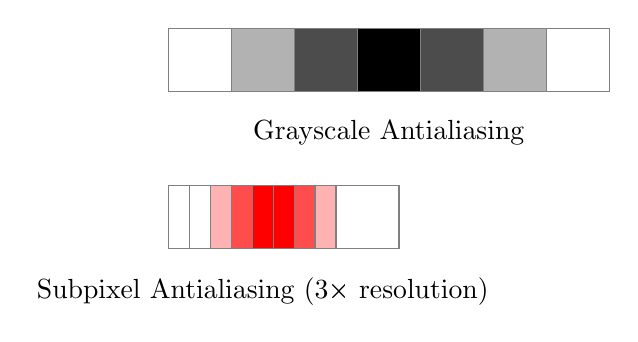
\begin{tikzpicture}[scale=0.8]
  % Traditional grayscale antialiasing
  \begin{scope}
    \foreach \x/\col in {0/0, 1/30, 2/70, 3/100, 4/70, 5/30, 6/0} {
      \fill[black!\col] (\x,0) rectangle +(1,1);
      \draw[gray] (\x,0) rectangle +(1,1);
    }
    \node[below] at (3.5,-0.3) {Grayscale Antialiasing};
  \end{scope}
  
  % Subpixel rendering
  \begin{scope}[yshift=-2.5cm]
    \foreach \x/\r/\g/\b in {
      0/0/0/0,
      1/0/10/30,
      2/30/50/70,
      3/70/90/100,
      4/100/100/100,
      5/100/90/70,
      6/70/50/30,
      7/30/10/0,
      8/0/0/0
    } {
      \fill[red!\r] (\x*0.333,0) rectangle +(0.333,1);
      \fill[green!\g] (\x*0.333+0.333,0) rectangle +(0.333,1);
      \fill[blue!\b] (\x*0.333+0.666,0) rectangle +(0.333,1);
      \draw[gray,thin] (\x*0.333,0) rectangle +(0.999,1);
    }
    \node[below] at (1.5,-0.3) {Subpixel Antialiasing (3× resolution)};
  \end{scope}
\end{tikzpicture}
\caption{Comparison of grayscale vs subpixel antialiasing. Subpixel rendering achieves 3× horizontal resolution.}
\end{figure}

\subsection{Mathematical Model}

\begin{formulabox}{ClearType Algorithm}
\textbf{Step 1:} Generate oversampled grayscale image at 3× horizontal resolution

\textbf{Step 2:} Apply asymmetric filter $F$ accounting for subpixel order:
\begin{equation}
  F = [0.06, 0.24, 0.40, 0.24, 0.06] \quad \text{(normalized Gaussian)}
\end{equation}

\textbf{Step 3:} Distribute filtered values to RGB subpixels:
\begin{align}
  R(x,y) &= F_R(G_{\text{oversample}}) \\
  G(x,y) &= F_G(G_{\text{oversample}}) \\
  B(x,y) &= F_B(G_{\text{oversample}})
\end{align}
\end{formulabox}

\section{Implementation Considerations}

\begin{itemize}
  \item Requires knowledge of subpixel order (RGB vs BGR)
  \item Rotation-dependent (only works for horizontal text)
  \item Can introduce color fringes on high-contrast edges
  \item Ineffective on PenTile due to shared subpixels
\end{itemize}

\chapter{Fill Factor and Optical Efficiency}

\section{Definitions}

\begin{formulabox}{Key Metrics}
\textbf{Fill Factor:}
\begin{equation}
  \text{FF} = \frac{A_{\text{active}}}{A_{\text{total}}}
\end{equation}

\textbf{Aperture Ratio (LCD):}
\begin{equation}
  \text{AR} = \frac{A_{\text{transmitting}}}{A_{\text{total}}}
\end{equation}

\textbf{Typical Values:}
\begin{itemize}
  \item LCD: FF = 60--70\%, AR = 5--8\%
  \item OLED: FF = 70--85\%, AR = 100\% (emissive)
\end{itemize}
\end{formulabox}

\begin{figure}[H]
\centering
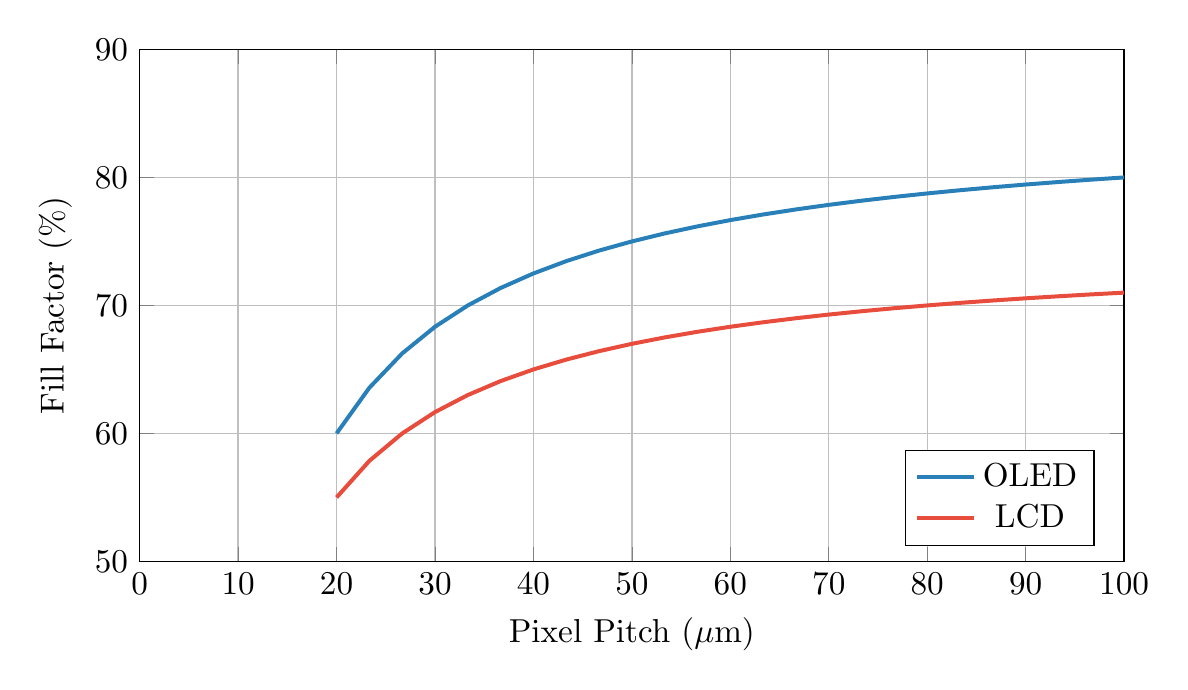
\begin{tikzpicture}[scale=1.2]
  \begin{axis}[
    width=12cm,
    height=7cm,
    xlabel={Pixel Pitch ($\mu$m)},
    ylabel={Fill Factor (\%)},
    xmin=0, xmax=100,
    ymin=50, ymax=90,
    grid=major,
    legend pos=south east
  ]
  
  % LCD fill factor decreases with smaller pixels
  \addplot[color=primarycolor, very thick, domain=20:100] 
    {85 - 500/x};
  \addlegendentry{OLED}
  
  \addplot[color=accentcolor, very thick, domain=20:100] 
    {75 - 400/x};
  \addlegendentry{LCD}
  
  \end{axis}
\end{tikzpicture}
\caption{Fill factor versus pixel pitch. Smaller pixels have lower fill factors due to fixed-size gaps and structures.}
\end{figure}

% Continue with many more chapters...

\chapter{Advanced Colorimetry}

\section{Color Gamut Visualization}

\begin{figure}[H]
\centering
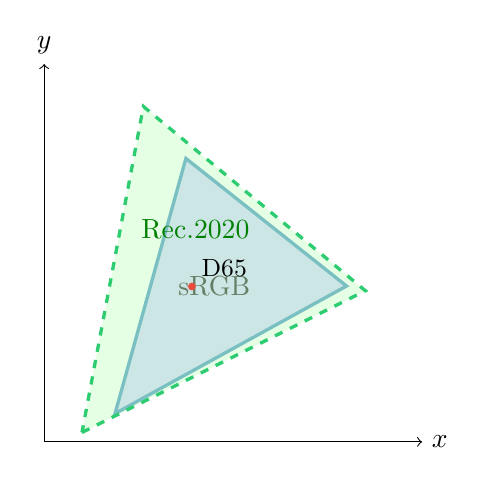
\begin{tikzpicture}[scale=6]
  % CIE 1931 chromaticity diagram (simplified)
  \fill[blue!20] (0.15,0.06) -- (0.64,0.33) -- (0.30,0.60) -- cycle;
  \draw[very thick, primarycolor] (0.15,0.06) -- (0.64,0.33) -- (0.30,0.60) -- cycle;
  \node at (0.36,0.33) {sRGB};
  
  \fill[green!20, opacity=0.5] (0.08,0.02) -- (0.68,0.32) -- (0.21,0.71) -- cycle;
  \draw[very thick, successcolor, dashed] (0.08,0.02) -- (0.68,0.32) -- (0.21,0.71) -- cycle;
  \node[green!50!black] at (0.32,0.45) {Rec.2020};
  
  \draw[->] (0,0) -- (0.8,0) node[right] {$x$};
  \draw[->] (0,0) -- (0,0.8) node[above] {$y$};
  
  \node[circle, fill=accentcolor, inner sep=1pt] at (0.3127,0.3290) {};
  \node[above right] at (0.3127,0.3290) {\small D65};
\end{tikzpicture}
\caption{CIE 1931 chromaticity diagram showing sRGB and Rec.2020 gamuts.}
\end{figure}

\section{RGB to XYZ Matrix Derivation}

\begin{formulabox}{Complete Derivation}
\textbf{Given:} RGB primary chromaticities and white point

\textbf{Step 1:} Construct primary matrix from chromaticities:
\begin{equation}
  P = \begin{bmatrix}
    x_r/y_r & x_g/y_g & x_b/y_b \\
    1 & 1 & 1 \\
    (1-x_r-y_r)/y_r & (1-x_g-y_g)/y_g & (1-x_b-y_b)/y_b
  \end{bmatrix}
\end{equation}

\textbf{Step 2:} White point in XYZ:
\begin{equation}
  \begin{bmatrix} X_w \\ Y_w \\ Z_w \end{bmatrix} = 
  \begin{bmatrix} x_w/y_w \\ 1 \\ (1-x_w-y_w)/y_w \end{bmatrix}
\end{equation}

\textbf{Step 3:} Scale factors:
\begin{equation}
  \begin{bmatrix} S_R \\ S_G \\ S_B \end{bmatrix} = 
  P^{-1} \begin{bmatrix} X_w \\ Y_w \\ Z_w \end{bmatrix}
\end{equation}

\textbf{Step 4:} Final RGB→XYZ matrix:
\begin{equation}
  M = P \cdot \text{diag}(S_R, S_G, S_B)
\end{equation}
\end{formulabox}

\chapter{HDR Tone Mapping}

\section{Global Tone Mapping Operators}

\subsection{Reinhard Operator}

\begin{formulabox}{Reinhard Tone Mapping}
\begin{equation}
  L_d = \frac{L \cdot (1 + L/L_{\text{white}}^2)}{1 + L}
\end{equation}

where:
\begin{itemize}
  \item $L$ = input luminance (HDR)
  \item $L_d$ = display luminance (SDR)
  \item $L_{\text{white}}$ = smallest luminance mapped to white
\end{itemize}
\end{formulabox}

\begin{figure}[H]
\centering
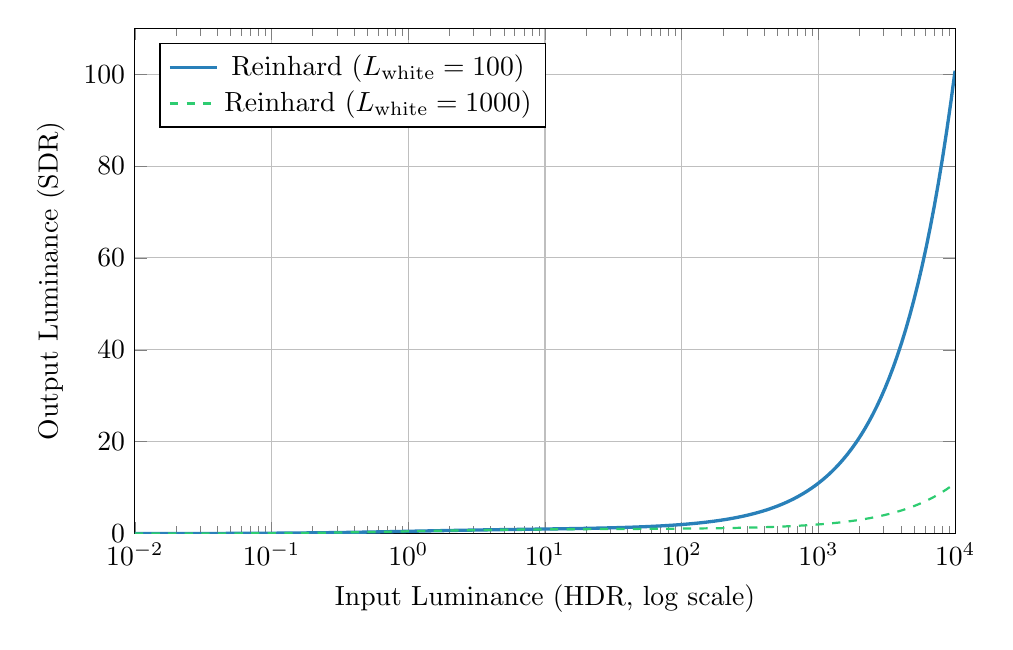
\begin{tikzpicture}
  \begin{axis}[
    width=12cm,
    height=8cm,
    xlabel={Input Luminance (HDR, log scale)},
    ylabel={Output Luminance (SDR)},
    xmode=log,
    xmin=0.01, xmax=10000,
    ymin=0, ymax=110,
    grid=major,
    legend pos=north west
  ]
  
  \addplot[color=primarycolor, very thick, domain=0.01:10000, samples=200] 
    {x*(1+x/100)/(1+x)};
  \addlegendentry{Reinhard ($L_{\text{white}}=100$)}
  
  \addplot[color=successcolor, thick, dashed, domain=0.01:10000, samples=200] 
    {x*(1+x/1000)/(1+x)};
  \addlegendentry{Reinhard ($L_{\text{white}}=1000$)}
  
  \end{axis}
\end{tikzpicture}
\caption{Reinhard tone mapping operator for different white points.}
\end{figure}

\chapter{Display Measurement and Calibration}

\section{Equipment Requirements}

\begin{table}[H]
\centering
\caption{Measurement Equipment Comparison}
\begin{tabular}{@{}llll@{}}
\toprule
\textbf{Property} & \textbf{Colorimeter} & \textbf{Spectroradiometer} & \textbf{Spot Meter} \\
\midrule
Accuracy & Fair & Excellent & Good \\
Speed & Fast & Slow & Fast \\
Cost & \$200--1000 & \$5000--30000 & \$500--2000 \\
Spectral data & No & Yes & No \\
Best for & Calibration & Research & Field work \\
\bottomrule
\end{tabular}
\end{table}

\section{Calibration Procedure}

\begin{algorithm}[H]
\caption{Display Calibration Workflow}
\begin{algorithmic}[1]
\State \textbf{Input:} Target white point, gamma, luminance
\State \textbf{Output:} LUT (Look-Up Table)
\State
\State Warm up display for 30+ minutes
\State Measure native white point and primaries
\For{each gray level $i = 0$ to 255}
  \State Display gray patch $i$
  \State Measure luminance $L_{\text{measured}}$
  \State Calculate $L_{\text{target}} = L_{\max} \cdot (i/255)^{\gamma}$
  \State $\text{LUT}[i] = \text{inverse}(L_{\text{target}})$
\EndFor
\State Apply LUT to display
\State Verify with test patterns
\end{algorithmic}
\end{algorithm}

\chapter{Manufacturing and Yield Optimization}

\section{Process Variations}

\begin{figure}[H]
\centering
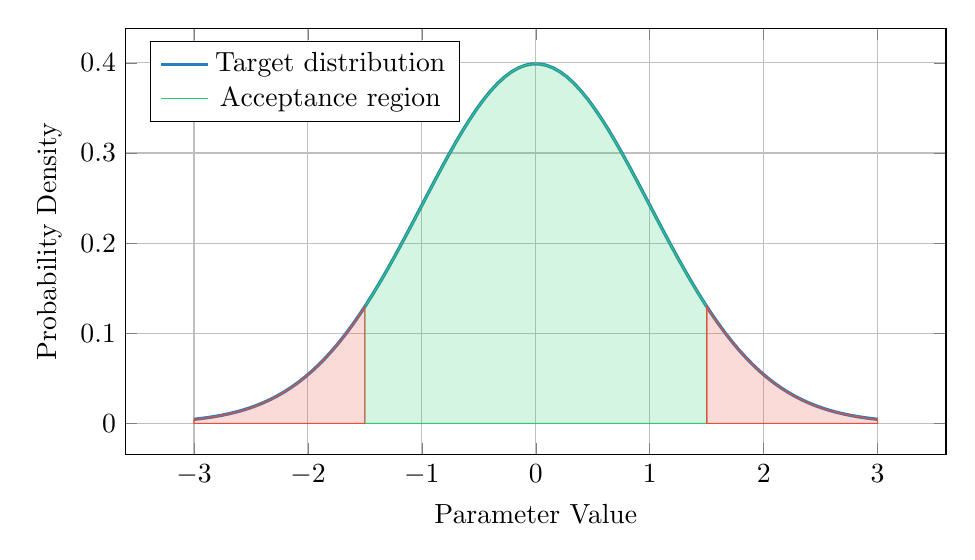
\begin{tikzpicture}
  \begin{axis}[
    width=12cm,
    height=7cm,
    xlabel={Parameter Value},
    ylabel={Probability Density},
    grid=major,
    legend pos=north west,
    domain=-3:3,
    samples=100
  ]
  
  % Normal distribution
  \addplot[color=primarycolor, very thick] 
    {exp(-x^2/2)/sqrt(2*pi)};
  \addlegendentry{Target distribution}
  
  % Acceptance region
  \addplot[color=successcolor, fill=successcolor, fill opacity=0.2, domain=-1.5:1.5] 
    {exp(-x^2/2)/sqrt(2*pi)} \closedcycle;
  \addlegendentry{Acceptance region};
  
  % Rejection regions
  \addplot[color=accentcolor, fill=accentcolor, fill opacity=0.2, domain=-3:-1.5] 
    {exp(-x^2/2)/sqrt(2*pi)} \closedcycle;
  \addplot[color=accentcolor, fill=accentcolor, fill opacity=0.2, domain=1.5:3] 
    {exp(-x^2/2)/sqrt(2*pi)} \closedcycle;
  
  \end{axis}
\end{tikzpicture}
\caption{Process variation and yield. Tighter tolerances reduce yield and increase cost.}
\end{figure}

\section{Cost-Performance Trade-offs}

\begin{formulabox}{Yield Model}
\textbf{Area-limited yield:}
\begin{equation}
  Y = e^{-AD}
\end{equation}

where:
\begin{itemize}
  \item $Y$ = yield (fraction of good devices)
  \item $A$ = device area
  \item $D$ = defect density (defects per unit area)
\end{itemize}

\textbf{Implications:}
\begin{itemize}
  \item Larger displays have exponentially lower yields
  \item Higher resolution (more area) reduces yield
  \item Defect reduction is critical for profitability
\end{itemize}
\end{formulabox}

\chapter{Power Management}

\section{OLED Power Modeling}

\begin{formulabox}{OLED Power Consumption}
\begin{equation}
  P_{\text{display}} = \eta \cdot A \cdot \langle L \rangle + P_{\text{base}}
\end{equation}

where:
\begin{itemize}
  \item $\eta$ = power efficiency coefficient (W·m²/cd)
  \item $A$ = display area (m²)
  \item $\langle L \rangle$ = average pixel luminance (cd/m²)
  \item $P_{\text{base}}$ = fixed power (driver, controller)
\end{itemize}

\textbf{Content dependence:}
\begin{itemize}
  \item White screen: Maximum power
  \item Black screen: Minimum power (near zero for OLED)
  \item Typical content: 30--50\% of maximum
\end{itemize}
\end{formulabox}

\begin{figure}[H]
\centering
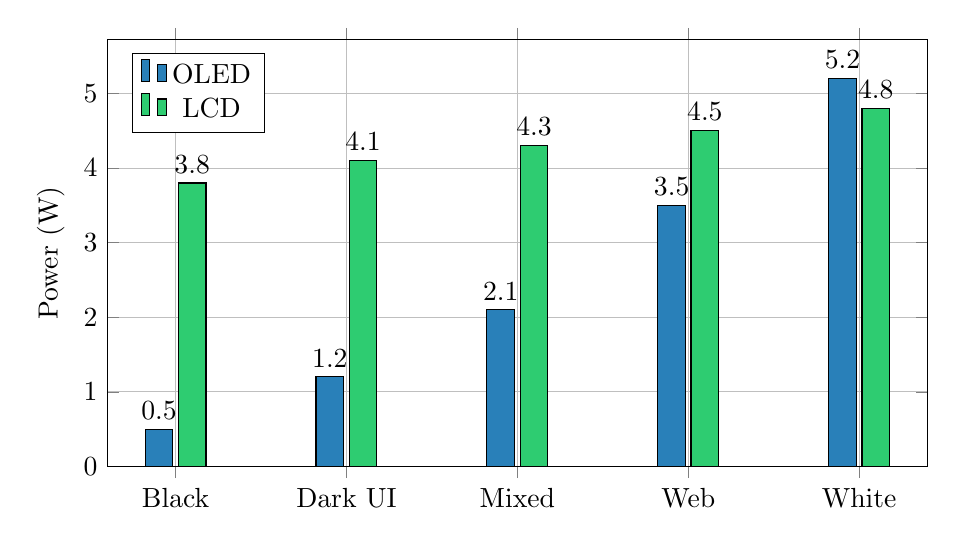
\begin{tikzpicture}
  \begin{axis}[
    ybar,
    width=12cm,
    height=7cm,
    ylabel={Power (W)},
    symbolic x coords={Black, Dark UI, Mixed, Web, White},
    xtick=data,
    nodes near coords,
    grid=major,
    ymin=0,
    legend pos=north west
  ]
  
  \addplot[fill=primarycolor] coordinates {
    (Black,0.5) (Dark UI,1.2) (Mixed,2.1) (Web,3.5) (White,5.2)
  };
  \addlegendentry{OLED}
  
  \addplot[fill=successcolor] coordinates {
    (Black,3.8) (Dark UI,4.1) (Mixed,4.3) (Web,4.5) (White,4.8)
  };
  \addlegendentry{LCD}
  
  \end{axis}
\end{tikzpicture}
\caption{Content-dependent power consumption for OLED vs LCD. LCD power is nearly constant (backlight), while OLED scales with content brightness.}
\end{figure}

\appendix
\chapter{Complete Formula Reference}

\begin{table}[H]
\centering
\caption{Core Equations Used Throughout This Text}
\label{tab:formula_reference}
\begin{tabular}{@{}lll@{}}
\toprule
\textbf{Topic} & \textbf{Equation} & \textbf{Primary Use} \\
\midrule
Display gamma & $L=L_{\max}V^{\gamma}$ & SDR response modeling \\
BT.1886 & $L=(aV+b)^{\gamma}$ & Reference EOTF with non-zero black \\
PQ EOTF & ST.2084 nonlinearity & Absolute HDR luminance mapping \\
HLG OETF & Piecewise sqrt/log & Broadcast HDR encoding \\
Chromaticity & $x=X/(X+Y+Z)$, $y=Y/(X+Y+Z)$ & Gamut/white-point work \\
Color difference & $\Delta E_{76}, \Delta E_{00}$ & Tolerance and quality control \\
Ambient veiling & $L_v\approx E_{\text{amb}}\rho/\pi$ & Contrast prediction in real rooms \\
\bottomrule
\end{tabular}
\end{table}

\chapter{Standard Illuminants}

\begin{table}[H]
\centering
\caption{Common CIE Illuminants in Display Workflows}
\label{tab:illuminants}
\begin{tabular}{@{}lccc@{}}
\toprule
\textbf{Illuminant} & \textbf{Description} & \textbf{Approx. CCT (K)} & \textbf{Typical Use} \\
\midrule
A & Tungsten/incandescent reference & 2856 & Legacy lamp simulation \\
D50 & Horizon daylight / warm daylight & 5003 & Print and ICC PCS workflows \\
D55 & Mid-morning daylight & 5503 & Photography reference sets \\
D65 & Noon daylight average & 6504 & sRGB/Rec.709/Rec.2020 white \\
D75 & Cool daylight & 7504 & Niche viewing conditions \\
\bottomrule
\end{tabular}
\end{table}

\chapter{Color Matching Functions}

The CIE 1931 2-degree color matching functions $\bar{x}(\lambda)$, $\bar{y}(\lambda)$, and $\bar{z}(\lambda)$ define the linear transform from spectra to XYZ tristimulus values. In practice:
\begin{itemize}
  \item $\bar{y}(\lambda)$ is aligned with photopic luminance sensitivity.
  \item Numerical integration is usually implemented as a weighted sum over sampled wavelengths.
  \item 10-degree observer data can be preferable for wide-field stimuli.
\end{itemize}

\backmatter
\bibliographystyle{plain}
% \bibliography{references}

\end{document}
